%------------------------------------------------------------------------------
% 
% by Quentin Bammey, Marina Gardella, Tina Nikoukhah, Miguel Colom, Jean-Michel Morel, Rafael Grompone von Gioi
%------------------------------------------------------------------------------
\documentclass{ipol}

\ipolSetTitle{Image Forgeries detection through Mosaic Analysis: the Intermediate Values Algorithm}
\ipolSetAuthors{Quentin Bammey, Rafael Grompone von Gioi, Jean-Michel Morel}

\ipolSetAffiliations{Universit\'e Paris-Saclay, ENS Paris-Saclay, CNRS, Centre Borelli, F-94235, Cachan, France \\
\texttt{\{quentin.bammey, rafael.grompone, jean-michel.morel\}@ens-paris-saclay.fr}}

%------------------------------------------------------------------------------
\ipolPreprintLink{https://ipolcore.ipol.im/demo/clientApp/demo.html?id=77777000095}

%------------------------------------------------------------------------------
\usepackage{subcaption}
\usepackage[dvipsnames, table]{xcolor}

%All the colours we used for the database articles. c0, c1, c2 and c3 go nicely together
\definecolor{c0}{HTML}{0E918C}
\definecolor{c1}{HTML}{F6830F}
\definecolor{c2}{HTML}{BB2205}
\definecolor{c3}{HTML}{1F3C88}
\definecolor{grayA}{HTML}{D2D3C9}
\definecolor{cgray}{HTML}{708090}
\definecolor{cgreen}{HTML}{1F8C88}

\usepackage{soul}
\sethlcolor{c0!50}

\usepackage[vlined,algoruled,linesnumbered]{algorithm2e}
\usepackage{namedinput}

\SetKwNamedIO{Input}{Input}
\SetKwNamedIO{Parameter}{Param}
\SetKwNamedIO{Output}{Output}
%\SetKwInOut{dontusethis}{aaaaaaaaaaaaaa}  % hack to get enough spacing for names
\renewcommand{\KwSty}[1]{\textnormal{\textcolor{c1}{\ttfamily\bfseries #1}}\unskip}
\renewcommand{\ArgSty}[1]{\textnormal{\ttfamily #1}\unskip}
\renewcommand{\DataSty}[1]{\color{c2}\bfseries #1}
\SetKwComment{Comment}{\color{c0}\# }{}
\renewcommand{\CommentSty}[1]{\textnormal{\ttfamily\color{c0}#1}\unskip}
\newcommand{\assign}{:\!=}
\newcommand{\peq}{+\mkern-8mu=}
\newcommand{\var}{\texttt}
\newcommand{\FuncCall}[2]{\texttt{\bfseries #1(#2)}}
\SetKwProg{Function}{function}{}{}
\renewcommand{\ProgSty}[1]{\texttt{\bfseries \color{c3}#1}}
\DontPrintSemicolon
\SetKw{IN}{in}
\SetKw{AND}{and}
\SetKw{FROM}{from}
\SetKw{TO}{to}
%\newcommand{\IN}{~\KwSty{in}~}
%\newcommand{\FROM}{~\KwSty{from}~}
%\newcommand{\TO}{~\KwSty{to}~}
\usepackage{booktabs} % table
\usepackage{multirow}
\usepackage{array}
\usepackage{tikz}
\usepackage{amsmath, amssymb}
\DeclareMathOperator*{\argmax}{arg\,max}

%\renewcommand*{\thesubfigure}{(\thefigure.\arabic{subfigure})}
%------------------------------------------------------------------------------
\newcommand{\qb}[1]{\textcolor{c1}{(Quentin) #1}}

\begin{document}


\begin{ipolAbstract}
        Camera only sample images in one colour channel per pixel. The remaining channels are interpolated from neighbouring pixels during demosaicing. This operation leaves traces, that can be exploited to authentify images and detect forgeries. This paper describes a method that exploits the fact that interpolated pixels are more prone to be intermediate values to detect in which pattern an image has been sampled. We then use this information to find regions that are inconsistent with the global image. We attribute a confidence score to each detection, which can then be thresholded to provide a binary map of detected forgeries.
\end{ipolAbstract}

\begin{ipolCode}
The reviewed source code and documentation for this algorithm are
available from \href{\ipolLink}{the web page of this
article}. Usage instruction are included in the
\verb|README.txt| file of the archive.
\end{ipolCode}

\begin{ipolSupp}
The link to the demo is \href{https://ipolcore.ipol.im/demo/clientApp/demo.html?id=77777000095}{https://ipolcore.ipol.im/demo/clientApp/demo.html?id=77777000095}.
\end{ipolSupp}

\ipolKeywords{image forensics, forgery detection}
\newpage

%------------------------------------------------------------------------------
\section{Introduction}

\begin{figure}[ht]
        \centering
        \begin{subfigure}{.4\linewidth}
                \centering
                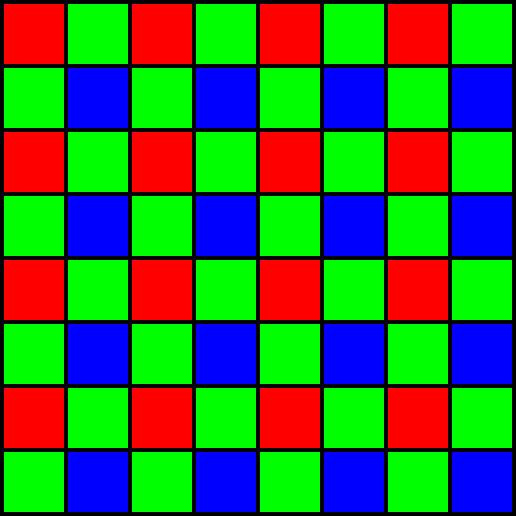
\includegraphics[width=.6\linewidth]{images/cfa.png}
                \label{fig:bayer}
                \caption{The Bayer CFA, by far the most commonly used CFA}
        \end{subfigure}\hfill%
        \begin{subfigure}{.6\linewidth}
                \centering
                \begin{tabular}{cc}
                        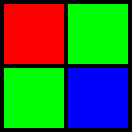
\includegraphics[width=40pt]{images/rggb.png}&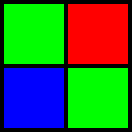
\includegraphics[width=40pt]{images/grbg.png}\\
                        \textsc{rggb}&\textsc{grbg}\\
                        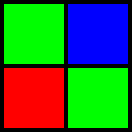
\includegraphics[width=40pt]{images/gbrg.png}&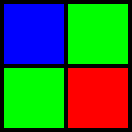
\includegraphics[width=40pt]{images/bggr.png}\\
                        \textsc{gbrg}&\textsc{bggr}\\
                \end{tabular}
                \label{fig:4patterns}
                \caption{The four potential patterns that arise from the Bayer CFA.}
        \end{subfigure}
        \caption{The Bayer Colour Filter Array(CFA), and the four potential patterns that arise from it. The pattern identifies the position of the top-left red-sampled pixel in an image.}
\end{figure}

Most cameras cannot see true colour images. They can only sample one colour per pixel using a colour filter array (CFA), and must interpolate the missing values. The most common CFA is the Bayer matrix, shown in Figure~\ref{fig:bayer}. It is made of a simple $2\times2$ pattern, which samples twice as many pixels in green as in red or blue. Because interpolation leaves traces, it is sometimes possible to identify in which pattern an image has been sampled, in other words, to know which of the four blocks seen in Figure~\ref{fig:4patterns} represent the first sampled pixels at the image origin.

If there is a forgery in an images, chances are the pattern in the manipulated area will not coincide with the rest of the image. For instance, if part of an image is copied and pasted onto another (or potentially the same) image, there is a $\frac34$ chance that the patterns will not be aligned, as can be seen in Figure~\ref{fig:forgeryshift}. If this shift in the periodic pattern of sampled colours can be detected, then it will consitute an important evidence as to the presence of a forgery.

\begin{figure}[ht]
        \centering
        \begin{subfigure}{.5\linewidth}
                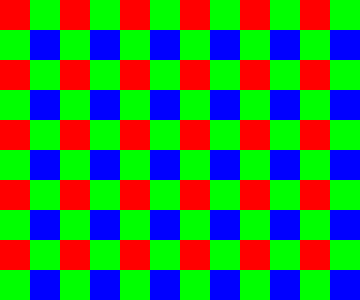
\includegraphics[width=.9\linewidth]{images/bayer.png}
                \caption{Authentic image}
        \end{subfigure}\hfill%
        \begin{subfigure}{.5\linewidth}
                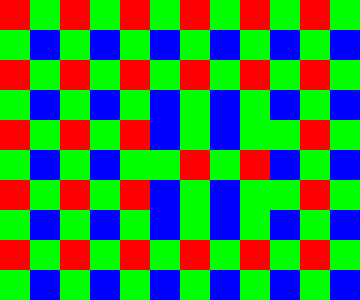
\includegraphics[width=.9\linewidth]{images/bayer_forged.png}
                \caption{Forged image}
        \end{subfigure}
        \label{fig:forgeryshift}
        \caption{Colours in which pixels are sampled in an authentic and forged image. In the forged area of the second image, there is a $\frac34$ probability that the patterns of the authentic and forged area are misaligned, causing a shift in the otherwise-periodic CFA.}
\end{figure}

The method we present here, originally proposed by Choi et al.~\cite{choi}, uses the fact that demosaicing is basically an interpolation operation. As a consequence, interpolated pixels are more often intermediate values between among their immediate neighbours, as seen in Figure~\ref{fig:intermediate_values}. For instance, with the simple bilinear demosaicing, missing colours are directly averaged from the direct neighbours that were originally sampled in that colour, and are thus always intermediate values. 

\begin{figure}[ht]
        \centering
        \begin{subfigure}[t]{.5\linewidth}
                \centering
                \begin{tabular}{cccccccccc}
                        18 & \textcolor{c2}{56} & 94 & \textcolor{c2}{85} & 76 & \textcolor{c2}{96} & 116 & \textcolor{c2}{104}\\
                        \textcolor{c2}{49} & \cellcolor{c0!50}{\textcolor{c2}{56}} & \cellcolor{c0!50}{\textcolor{c2}{63}} & \cellcolor{c0!50}{\textcolor{c2}{52}} & \cellcolor{c0!50}{\textcolor{c2}{41}} & \cellcolor{c0!50}{\textcolor{c2}{64}} & \cellcolor{c0!50}{\textcolor{c2}{88}} & \textcolor{c2}{87}\\
                        80 & \cellcolor{c0!50}{\textcolor{c2}{56}} & \cellcolor{c0!50}{32} & \cellcolor{c0!50}{\textcolor{c2}{19}} & 6 & \cellcolor{c0!50}{\textcolor{c2}{33}} & \cellcolor{c0!50}{60} & \textcolor{c2}{70}\\
                        \textcolor{c2}{59} & \cellcolor{c0!50}{\textcolor{c2}{62}} & \cellcolor{c0!50}{\textcolor{c2}{66}} & \cellcolor{c0!50}{\textcolor{c2}{49}} & \cellcolor{c0!50}{\textcolor{c2}{32}} & \cellcolor{c0!50}{\textcolor{c2}{59}} & \cellcolor{c0!50}{\textcolor{c2}{87}} & \textcolor{c2}{88}\\
                        38 & \cellcolor{c0!50}{\textcolor{c2}{69}} & 100 & \cellcolor{c0!50}{\textcolor{c2}{79}} & \cellcolor{c0!50}{58} & \cellcolor{c0!50}{\textcolor{c2}{86}} & 114 & \textcolor{c2}{106}\\
                        \textcolor{c2}{40} & \cellcolor{c0!50}{\textcolor{c2}{51}} & \cellcolor{c0!50}{\textcolor{c2}{63}} & \cellcolor{c0!50}{\textcolor{c2}{74}} & \cellcolor{c0!50}{\textcolor{c2}{85}} & \cellcolor{c0!50}{\textcolor{c2}{75}} & \cellcolor{c0!50}{\textcolor{c2}{66}} & \textcolor{c2}{63}\\
                        42 & \cellcolor{c0!50}{\textcolor{c2}{34}} & 26 & \cellcolor{c0!50}{\textcolor{c2}{69}} & 112 & \cellcolor{c0!50}{\textcolor{c2}{65}} & 18 & \textcolor{c2}{21}\\
                        \textcolor{c2}{38} & \textcolor{c2}{47} & \textcolor{c2}{57} & \textcolor{c2}{75} & \textcolor{c2}{94} & \textcolor{c2}{72} & \textcolor{c2}{50} & \textcolor{c2}{35}\\
                \end{tabular}
                \caption{Red channel}
        \end{subfigure}\hfill%
        \begin{subfigure}[t]{.5\linewidth}
                \centering
                \begin{tabular}{cccccccccc}
                    \textcolor{c2}{139} & 240 & \textcolor{c2}{154} & 16 & \textcolor{c2}{94} & 56 & \textcolor{c2}{72} & 20\\
                    92 & \cellcolor{c0!50}{\textcolor{c2}{131}} & 168 & \cellcolor{c0!50}{\textcolor{c2}{76}} & 72 & \cellcolor{c0!50}{\textcolor{c2}{94}} & 24 & \textcolor{c2}{43}\\
                    \textcolor{c2}{85} & 24 & \cellcolor{c0!50}{\textcolor{c2}{100}} & 48 & \cellcolor{c0!50}{\textcolor{c2}{102}} & 224 & \cellcolor{c0!50}{\textcolor{c2}{130}} & 72\\
                    60 & \cellcolor{c0!50}{\textcolor{c2}{107}} & 160 & \cellcolor{c0!50}{\textcolor{c2}{68}} & \cellcolor{c0!50}{64} & \cellcolor{c0!50}{\textcolor{c2}{122}} & 200 & \textcolor{c2}{153}\\
                    \textcolor{c2}{92} & 184 & \cellcolor{c0!50}{\textcolor{c2}{125}} & 0 & \cellcolor{c0!50}{\textcolor{c2}{50}} & 0 & \cellcolor{c0!50}{\textcolor{c2}{133}} & 108\\
                    52 & \cellcolor{c0!50}{\textcolor{c2}{155}} & 156 & \cellcolor{c0!50}{\textcolor{c2}{76}} & 136 & \cellcolor{c0!50}{\textcolor{c2}{117}} & 224 & \textcolor{c2}{127}\\
                    \textcolor{c2}{146} & 228 & \cellcolor{c0!50}{\textcolor{c2}{111}} & 12 & \cellcolor{c0!50}{\textcolor{c2}{110}} & \cellcolor{c0!50}{108} & \cellcolor{c0!50}{\textcolor{c2}{107}} & 44\\
                    56 & \textcolor{c2}{114} & 48 & \textcolor{c2}{90} & 184 & \textcolor{c2}{141} & 52 & \textcolor{c2}{90}\\
                \end{tabular}
                \caption{Green channel}
        \end{subfigure}
        \label{fig:intermediate_values}
        \caption{Red and green channels of a toy image demosaiced with bilinear interpolation in the \textsc{rggb} pattern. \textcolor{c2}{Red values} correspond to positions where the value was interpolated. \hl{Highlighted} cells correspond to pixels that take an intermediate value, ie.\@ that are not a local extrema among their direct neighbourhood. While sampled pixels can have intermediate values, many more can be found among \textcolor{c3}{interpolated pixels} in both the red and green channel. The blue channel, not shown here, behave similarly to the red one.}
\end{figure}

Of course, this certainty is no longer true with more complex algorithms, which interpolate pixels using further samples and across channels. Nevertheless, with most algorithms, an interpolated pixel is still more likely to be an intermediate value than a sampled one.

In this paper, we describe, analyze and expand this method.
The original article explains how to detect in which pattern an image, or part of it, has been sampled. Starting from there, we detect which regions of an image are inconsistent with the main image, and attribute a confidence score to this detection.
We also propose another way of computing intermediate values, which yields slightly better results. 

%------------------------------------------------------------------------------
\section{Method}
During demosaicing, missing colours on each pixel are interpolated from its neighbours. As a consequence, pixels that are interpolated in a given channel are more likely to be an intermediate value, in other words, to be neither lower than all its direct neighbours nor higher than all of them. This is especially true with the most simple demosaicing algorithm, such as bilinear demosaicing which interpolate the three channels separately.

This method proposes to count the intermediate values corresponding to each of the four patterns. On the correct pattern, as most pixels are sampled, there should be fewer intermediate values than in the other patterns.

\subsection{Intermediate values detection}
Let $I$ of shape $(X, Y)$ be one colour channel of an image. The pixel at location $(x, y)$ is considered an intermediate value if $\min(I_{x-1, y}, I_{x+1, y}, I_{x, y-1}, I_{x, y+1}) \leq I_{x, y} \leq \max(I_{x-1, y}, I_{x+1, y}, I_{x, y-1}, I_{x, y+1})$.

We define $\mathcal M(I)$ as the mask of intermediate values of $I$. We define it as 1 if $(x, y)$ is an intermediate value of $I$, and $0$ otherwise.

On the border of the image, either $x\pm1$ or $y\pm1$ is out of the image boundaries. To avoid border effects, we would thus have to mask out a 1-pixel border around the image. However, doing this would cause an imbalance in the number of pixels corresponding to different patterns, in other words their would be, in border windows, more pixels corresponding to one pattern than another. To solve the imbalance, we instead mask out a 2-pixels-wide border.

More formally, the mask of intermediate values is thus defined as:
\[\phantom.\mathcal M(I)_{x, y} \triangleq \left\{\begin{array}{ll}
        0 &\text{if }x\in\{0, 1, X-2, X-1\}\text{ or }y\in\{0, 1, Y-2, Y-1\}\\
        1 &\text{otherwise, if}\min(I_{x-1, y}, I_{x+1, y}, I_{x, y-1}, I_{x, y+1}) \leq I_{x, y} \leq \max(I_{x-1, y}, I_{x+1, y}, I_{x, y-1}, I_{x, y+1})\\
0 &\text{otherwise}\end{array}\right.\]
The computation of this mask is described in Algorithm~\ref{alg:intermediate}.

Furthermore, to limit demosaicing artefacts, many demosaicing algorithm tend to avoid interpolating against strong gradients, such as against an edge, and thus often only interpolate in one direction (in which the gradient is smaller). To take this into account, we propose to replace the original isotropic intermediate values mask with bidirectional filters, that separately considers horizontally and vertically intermediate values. We define the mask of horizontal intermediate values as
\[\phantom.\mathcal M(I)^h_{x, y} \triangleq \left\{\begin{array}{ll}
        0 &\text{if }x\in\{0, 1, X-2, X-1\}\text{ or }y\in\{0, 1, Y-2, Y-1\}\\
        1 &\text{otherwise, if}\min(I_{x-1, y}, I_{x+1, y}) \leq I_{x, y} \leq \max(I_{x-1, y}, I_{x+1, y})\\
0 &\text{otherwise}\end{array}\right..\]
Vertical values are computed in a similar way:
\[\phantom.\mathcal M(I)^v_{x, y} \triangleq \left\{\begin{array}{ll}
        0 &\text{if }x\in\{0, 1, X-2, X-1\}\text{ or }y\in\{0, 1, Y-2, Y-1\}\\
        1 &\text{otherwise, if}\min(I_{x, y-1}, I_{x, y+1}) \leq I_{x, y} \leq \max(I_{x, y-1}, I_{x, y+1})\\
0 &\text{otherwise}\end{array}\right..\]
Under this definition, the bidirectional mask of intermediate values is then defined as the mean of the horizontal and vertical masks:
\[\phantom.\mathcal M(I)_{x, y} \triangleq\frac 1 2 \left(M(I)^h_{x, y} + M(I)^v_{x, y}\right).\]
It is thus null at the border and where a pixel is not an intermediate value, equal to $\frac 1 2$ where the pixel is either horizontally or vertically an intermediate value, and equal to $1$ when it is an intermediate value both horizontally and vertically. The computation of the isotropic mask is detailed in Algorithm~\ref{alg:intermediate_bidirectional}.

The original isotropic mask and the bidirectional one will be compared in Section~\ref{sec:experiments}. For the rest of this section, we consider $R$, $G$ and $B$ the masks of intermediate values obtained on the respectively red, green and blue channels of the image. Which of the two methods was used to compute those masks is irrelevant to the rest of the algorithm.

\begin{algorithm}[h]
\caption{Mark intermediate values (original isotropic version)}
\label{alg:intermediate}
\Function{is\_intermediate(arr)}{
\Input{arr}{Array of size $(X, Y)$, one channel of an image}
\Output{mask}{Array of size $(X-4, Y-4)$, intermediate values mask}

mask $\assign \mathbf 0_{(X-4, Y-4)}$\;
\For{$x$ \FROM 2 \TO $X-2$ \AND $y$ \FROM 2 \TO $Y-2$}{
$\mathrm{mi}\assign \min{(\mathrm{arr}_{x+1, y}, \mathrm{arr}_{x, y-1}, \mathrm{arr}_{x-1, y}, \mathrm{arr}_{x, y+1})}$\;
$\mathrm{ma}\assign \max{(\mathrm{arr}_{x+1, y}, \mathrm{arr}_{x, y-1}, \mathrm{arr}_{x-1, y}, \mathrm{arr}_{x, y+1})}$\;
\If{$\mathrm{mi} \leq \mathrm{arr}_{x, y} \leq \mathrm{ma}$}
{
    $\mathrm{mask}_{x-2, y-2}\assign 1$\;
}
}
\Return{mask}
}
\end{algorithm}

\begin{algorithm}[h]
\caption{Mark intermediate values (bidirectional variant)}
\label{alg:intermediate_bidirectional}
\Function{is\_intermediate(arr)}{
\Input{arr}{Array of size $(X, Y)$, one channel of an image}
\Output{mask}{Array of size $(X-4, Y-4)$, intermediate values mask}

mask $\assign \mathbf 0_{(X-4, Y-4)}$\;
\For{$x$ \FROM 2 \TO $X-2$ \AND $y$ \FROM 2 \TO $Y-2$}{
        $\mathrm{mi}_h\assign \min(\mathrm{arr}_{x-1, y}, \mathrm{arr}_{x+1, y})$\;
        $\mathrm{ma}_h\assign \max(\mathrm{arr}_{x-1, y}, \mathrm{arr}_{x+1, y})$\;
        $\mathrm{mi}_v\assign \min(\mathrm{arr}_{x, y-1}, \mathrm{arr}_{x, y+1})$\;
        $\mathrm{ma}_v\assign \max(\mathrm{arr}_{x, y-1}, \mathrm{arr}_{x, y+1})$\;

\If{$\mathrm{mi_h} \leq \mathrm{arr}_{x, y} \leq \mathrm{ma_h}$}
{
    $\mathrm{mask}_{x-2, y-2}\peq \frac 1 2$\;
}
\If{$\mathrm{mi_v} \leq \mathrm{arr}_{x, y} \leq \mathrm{ma_v}$}
{
    $\mathrm{mask}_{x-2, y-2}\peq \frac 1 2$\;
}
}
\Return{mask}
}
\end{algorithm}

\subsection{Division into windows}
The strategy to find forgeries using inconsistencies in the CFA patterns is to first find in which pattern the full image has been demosaiced, then to find the pattern used in different windows of the image. If a the pattern detected in a window is different than the one detected for the full image, then this window is inconsistent with the rest of the image and can be considered as forged.

To improve the precision of detection, we do not simply use adjacent windows, but rather sliding windows with an overlap. The window size $W$ and stride are set as parameters of the algorithm. The stride determines the number of pixel between the left (or top) border of two consecutive windows, such as a stride equal to the window size leads to adjacent windows without overlapping, a stride equal to half the window size leads to a new window starting at the middle of the previous one, etc.

Using a lower stride will not drastically improve the detection, but may help contour a detected forgery more precisely, at the cost of a slower algorithm.

In the rest of this section, we consider the windowed intermediate values as of shape $(X_w, Y_w, 3, W, W)$, where $X_w$ and $Y_w$ are the number of windows in a row and in a column. In practice, the windows are computed in one dimension, and the full array is thus of shape $(X_w*Y_w, 3, W, W)$, and is only reshaped at the end of the computation.

\subsection{Finding the pattern}
\begin{figure}[h]
        \centering
        \begin{tabular}{ccccc}
                \multicolumn{2}{c}{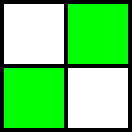
\includegraphics[width=30pt]{images/xggx.png}}&&\multicolumn{2}{c}{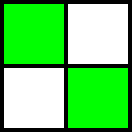
\includegraphics[width=30pt]{images/gxxg.png}}\\
                \multicolumn{2}{c}{\textsc{·gg·}} && \multicolumn{2}{c}{\textsc{g··g}}\\
                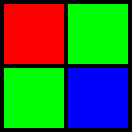
\includegraphics[width=30pt]{images/rggb.png}&
                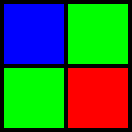
\includegraphics[width=30pt]{images/bggr.png}&
                \qquad\qquad& %ugly hack I know
                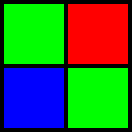
\includegraphics[width=30pt]{images/grbg.png}&
                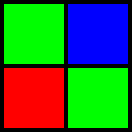
\includegraphics[width=30pt]{images/gbrg.png}\\
                \textsc{rggb} & \textsc{bggr} && \textsc{grbg} & \textsc{gbrg}\\
        \end{tabular}
        \label{fig:fourpatterns}
        \caption{The four possible sampling patterns can be grouped by the diagonal on which the green channel was sampled: \textsc{rggb} and \textsc{bggr} share the \textsc{·gg·} diagonal, whereas \textsc{grbg} and \textsc{gbrg} share the \textsc{g··g} one.}
\end{figure}
The four patterns can be divided into two subgroups by their diagonal: \textsc{rggb} and \textsc{bggr} share the \textsc{·gg·} diagonal, whereas \textsc{grbg} and \textsc{gbrg} share the \textsc{g··g} diagonal. Because the Bayer CFA samples twice as many pixels in green than in red or blue, it is easier to find information on the pattern in the green channel. This is amplified by the fact that many demosaicing algorithms first interpolate the green channel by itself, but interpolate the red and blue channels using information from the green channel.

As a consequence, the presented method first tries to detect the diagonal pattern using the green channel(\textsc{·gg·} or \textsc{g··g}), then uses the red and blue channels to compare the two potential patterns sharing that diagonal.

Let $R$, $G$ and $B$ be the masks of intermediate values on the respectively red, green and blue channels, These masks, each of shape $(2X, 2Y)$, can represent either the full image or a window of it. To maintain the balance between patterns, those masks must be of even size. For this reasons, the window size must be even, and the last row/column of the full image is removed if necessary to ensure the evenness of the shape

We start by looking at the green channel for the diagonal grids. The intermediate value count corresponding to the \textsc{·gg·} pattern is
\[C_{\textsc{·gg·}} \triangleq \sum_{x=0}^X\sum_{y=0}^Y\left(G_{2x+1, 2y} + G_{2x, 2y+1}\right)\]
while the count corresponding to the \textsc{g··g} pattern is
\[\phantom.C_{\textsc{g··g}} \triangleq \sum_{x=0}^X\sum_{y=0}^Y\left(G_{2x, 2y} + G_{2x+1, 2y+1}\right).\]

The count difference of the diagonal is then defined as
\[\phantom.\Delta_{\mathrm{diag}}  \triangleq \frac 1 {2X\cdot Y} \left(C_{\textsc{·gg·}} - C_{\textsc{g··g}}\right)\]
This difference is positive if the detected diagonal is \textsc{g··g}, and negative if it is \textsc{·gg·}:
\[\phantom.D\triangleq\left\{\begin{array}{lc}\textsc{g··g}&\Delta_{\mathrm{diag}}>0\\\textsc{·gg·}&\Delta_{\mathrm{diag}}>0\\-1&\text{otherwise}\end{array}\right..\]
        The normalization by $\frac{1}{2XY}$ means that the resulting difference is in $[-1, 1]$, and is equal to $\pm1$ if all pixels in one of the patterns are intermediate values, whereas the other pattern has no intermediate values--~$XY$ is the number of $2\times2$ blocks in a mask of shape $(2X, 2Y)$, and we sum two pixels in this block for each pattern. Note that the $\pm1$ limit is only theoretical: Even with bilinear demosaicing, where all interpolated pixels are intermediate values, sampled pixels can be intermediate too, eg.\@ in a slope. As a consequence, the difference will not reach those values in natural cases.

Once we know the main diagonal, we can compare the two patterns sharing that diagonal. The green channel does not provide any information on this, so we use the red and blue channels.

The count of intermediate values corresponding to each pattern is:
\[\phantom.\begin{array}{ll}
        C_{\textsc{rggb}} &\triangleq \sum_{x=0}^X\sum_{y=0}^Y\left(R_{2x, 2y} + B_{2x+1, 2y+1}\right)\\
        C_{\textsc{bggr}} &\triangleq \sum_{x=0}^X\sum_{y=0}^Y\left(R_{2x+1, 2y+1} + B_{2x, 2y}\right)\\
        C_{\textsc{grbg}} &\triangleq \sum_{x=0}^X\sum_{y=0}^Y\left(R_{2x+1, 2y} + B_{2x, 2y+1}\right)\\
        C_{\textsc{gbrg}} &\triangleq \sum_{x=0}^X\sum_{y=0}^Y\left(R_{2x, 2y+1} + B_{2x+1, 2y}\right)
\end{array}.\]

The count differences of the two pattern pairs are then defined as
\[\begin{array}{ll}
        \Delta_{\textsc{rggb}-\textsc{bggr}} &\triangleq \frac 1 {2XY}\left( C_{\textsc{rggb}} - C_{\textsc{bggr}}\right)\\
\Delta_{\textsc{grbg}-\textsc{gbrg}} &\triangleq \frac 1 {2XY}\left(C_{\textsc{rggb}} - C_{\textsc{gbrg}}\right)\end{array}\]
and are then combined into the main grid difference
\[\phantom.\Delta_{\mathrm{main}}\triangleq\left\{\begin{array}{lc}
        \Delta_{\textsc{rggb}-\textsc{bggr}}&D=\textsc{g··g}\\
\Delta_{\textsc{grbg}-\textsc{gbrg}}&D=\textsc{·gg·}\end{array}\right..\]
Finally, the main detected grid can be obtained:
\[\phantom.M \triangleq \left\{\begin{array}{lc}
        \textsc{rggb}&D=\textsc{·gg·}\text{ and }\Delta_{\mathrm{main}}<0\\
        \textsc{bggr}&D=\textsc{·gg·}\text{ and }\Delta_{\mathrm{main}}>0\\
        \textsc{grbg}&D=\textsc{g··g}\text{ and }\Delta_{\mathrm{main}}<0\\
        \textsc{gbrg}&D=\textsc{g··g}\text{ and }\Delta_{\mathrm{main}}>0\\
-1&\text{otherwise}\end{array}\right..\]

Both for the diagonal and main grids, if there is strict equality in the two counts detected, no grid is considered detected. Naturally, if no decision is taken on the diagonal, no main grid is selected either.

The grid detection is detailed in Algorithm~\ref{alg:grid}.

While $\Delta_{\mathrm{main}}$ is later used to make the decisions on forgeries, the two intermediary comparisons $\Delta_{\textsc{rggb}-\textsc{bggr}}$ and $\Delta_{\textsc{grbg}-\textsc{gbrg}}$ are easier to understand visually, and are thus kept for visualization.

Our implementation of the count difference computation is slightly different from the description of the original article. In the original article, the difference is not normalised by $\frac 1 {2XY}$. More importantly, the difference is computed separately in the red and blue channels, and the strongest of the two is kept, whereas we use their sum.
The reason for this is that the original article only tries to classify in which pattern an image has been sampled, without considering how confident one can be in the detection, or how to use it to detect forgeries. When only considering classification of an image or window into the four patterns, both the original article and our implementation provide the same results. However, adding the normalization and summing the two channels makes it easier for us to also compute a confidence value for the detections, which will be described in the next subsection.

Finally, we note that even though this algorithm is presented for one window, the grid detection is in practice done on all windows simultaneously.

\begin{algorithm}[h]
\caption{Find the grid}
\label{alg:grid}
\Function{find\_grid(R, G, B)}
{
        \qb{TBD: reorder the final if blocks to follow what is explained and done (even though this is equivalent).}
\Input{R}{Array of even size $(2X, 2Y)$, typically as returned by \FuncSty{is\_intermediate} or a sub-window of it on the red channel}
\Input{G}{Same as above for the green channel}
\Input{B}{Same as above for the blue channel}
\Output{main}{CFA pattern identified by the function (one of \textsc{rggb}, \textsc{grbg}, \textsc{gbrg}, \textsc{bggr})}
\Output{diag}{Diagonal pattern identified by the function (either \textsc{·gg·} or \textsc{g··g})}
\Output{diff\_main}{Difference of count in intermediate values between the two pattern sharing the same diagonal. Positive if the best pattern is \textsc{rggb} or \textsc{grbg}, negative if the best pattern is \textsc{gbrg} or \textsc{bggr}.}
\Output{diff\_diag}{Difference of count of intermediate values between the two diagonal patterns.}
\Comment{First we select the best diagonal pattern using the green values}
        $\mathrm{count_{*GG*}}\assign \sum_{x=0}^X\sum_{y=0}^YG_{2x,2y+1} + G_{2x+1, 2y}$\;
        $\mathrm{count_{G**G}}\assign \sum_{x=0}^X\sum_{y=0}^YG_{2x,2y} + G_{2x+1, 2y+1}$\;
$\mathrm{diff\_diag} \assign \frac 1{2XY}\left(\mathrm{count_{*GG*}} - \mathrm{count_{G**G}}\right)$\;
\If{$\mathrm{diff\_diag}$ < 0}{
diag$\assign$ \textsc{·gg·}\;
}
\Else{
diag$\assign$ \textsc{g··g}\;
}

\Comment{Now we select within the two patterns sharing the detected diagonal.}
\If{diff\_diag$=$\textsc{·gg·}}
{
\Comment{Either \textsc{rggb} or \textsc{bggr}}
        $\mathrm{count_{RGGB}}\assign \sum_{x=0}^{X}\sum_{y=0}^YR_{2x,2y} + B_{2x+1, 2y+1}$\;
        $\mathrm{count_{BGGR}}\assign \sum_{x=0}^X\sum_{y=0}^Y R_{2x+1,2y+1} + B_{2x, 2y}$\;
$\mathrm{diff\_main} \assign \frac 1{2XY}\left(\mathrm{count_{RGGB}} - \mathrm{count_{BGGR}}\right)$\;
\If{$\mathrm{diff\_main}$ < 0}{
main$\assign$ \textsc{rggb}\;
}
\Else{
main$\assign$ \textsc{bggr}\;
}
}
\Else
{
\Comment{Either \textsc{grbg} or \textsc{gbrg}}
$\mathrm{count_{GRBG}}\assign \sum_{x=0}^{\frac X 2}R_{2x+1,2y} + B_{2x, 2y+1}$\;
$\mathrm{count_{GBRG}}\assign \sum_{x=0}^{\frac X 2}R_{2x,2y+1} + B_{2x+1, 2y}$\;
$\mathrm{diff\_main} \assign \frac 2{XY}\left(\mathrm{count_{GRBG}} - \mathrm{count_{GBRG}}\right)$\;
\If{$\mathrm{diff\_main}$ < 0}{
main$\assign$ \textsc{grbg}\;
}
\Else{
main$\assign$ \textsc{gbrg}\;
}
}
\Return{main, diag, diff\_main, diff\_diag}
}
\end{algorithm}
\subsection{Forgery detection}
Using the previously-described algorithms, we can compute the intermediate value masks in all channels, cut them into windows, and detect the diagonal and pattern of the global image and of each window.

With this information, we could simply say that the windows which do not use the same pattern than the main grid correspond to forged regions. However, doing this creates many false positives, as the detection is not always correct.


%We do not propose here a way to automatically decide, without arbitrary parameters, which region to detect as forged. However, we show that a simple thresholding can filter out most of the false, noise-like positives, while keeping the relevant detections.
In first instance, if the grid of a window does not match the global image's grid, we can consider that window forged with a confidence of $|\Delta_{\mathrm{main}}|$ (or $|\Delta_{\mathrm{diag}}|$ if looking at the diagonals). However, if the threshold is low, isolated detections of a given grid will be detected by mistake. On the contrary, in a region with many windows sharing the same grid, only those above the threshold will be detected, so a high threshold will cause most of the detections to be missed. In both cases, using a fixed threshold will lead to mistakes that would be easy to avoid by looking at the map more globally.

We propose to segment the windows into connected components by their grids. In other words, a connected component is a set of spatially connected windows whose detected pattern is the same.
This segmentation is done with \texttt{scikit-image}~\cite{skimage}.

Components whose detected pattern is the global image's are immediately discarded; they are not considered forged as they are coherent with the full image.
For components whose detected pattern is different, we consider them as forged, with a confidence value which corresponds to the maximum absolute difference of count of all windows in that components (either $|\Delta_{\mathrm{main}}|$ or $|\Delta_{\mathrm{diag}}|$ depending on whether we are looking at the full pattern or the diagonal). In other words, the confidence of a component is that of the most prominent window it contains.

Applying this method to both the diagonal and the full pattern detections yields two confidence maps. We merge those two confidence maps into one by taking their pointwise maximum.

These confidence maps are useful to visualize the detection. However, they do not consitute by themselves a decision on the detection. They cannot either be used as a heatmap: the maximal absolute value of the difference, $1$, is never reached in actual cases, and even the most confident detections will rarely reach a score of $0.3$. 

To make a final decision on the image, we thus threshold the obtained confidence map by a given threshold $\gamma$. This is equivalent to performing hysteresis thresholding with a lower threshold 0 and a higher threshold $\gamma$ on each map $(M=g)\odot |\Delta_{\mathrm{main}}|$ for each pattern $g$ except the full image's pattern, and $(D\neq d_{\mathrm{img}})\odot|\Delta_{\mathrm{diag}}|$, where $d_{\mathrm{img}}$ is the full image's detected diagonal.
       

The computation of the forgery map is detailed in Algorithm~\ref{alg:global}. 

\begin{algorithm}[h]
        \caption{Global algorithm}
        \label{alg:global}
        \Function{find\_forgeries(img, W, stride, threshold)}
        {
                \Input{img}{Input image, size $(X, Y, 3)$}
                \Parameter{W}{int, Window size}
                \Parameter{stride}{int, Distance between the left/top border of two consecutive windows. Must divide W. If equal to it, windows will be adjacent without overlapping.}
                \Parameter{threshold}{float, higher hysteresis threshold to select relevant inconsistencies.}
                \Output{main, diag, diff\_main, diff\_diag}{Windowed output of \texttt{find\_grid}. See Alg.~\ref{alg:grid} for more details.}
                \Output{forged\_main, forged\_diag}{Windows whose detected / diagonal pattern is inconsistent with the global pattern}
                \Output{forged\_main\_thresholded, forged\_diag\_thresholded}{Same, after hysteresis thresholding}
                \Output{coords$_x$, coords$_y$}{Coordinates corresponding to the center of each window.}
                \Comment{Crop the image if needed, as $X$ and $Y$ need to be even.}
                $\mathrm{img} \assign \mathrm{img}[:X-X\%2, :Y-Y\%2]$\;
                $\mathrm{intermediate} \assign \mathtt{is\_intermediate}(\mathrm{img})$\;
                $\mathrm{windows}, \mathrm{coords_x}, \mathrm{coords_y} \assign \mathtt{get\_windows}(\mathrm{intermediate}, W, \mathrm{stride})$\;
                \Comment{Correct the coordinates to account for the lost border from \texttt{is\_intermediate}.}
                $\mathrm{coords_x}, \mathrm{coords_y} \peq 2$\;
                \Comment{Number of window rows and columns.}
                $X_w, Y_w \assign |\mathrm{coords_x}|, |\mathrm{coords_y}|$\;
                $\mathrm{global\_main}, \mathrm{global\_diag}, \_, \_ = \mathtt{find\_grid}(\mathrm{intermediate}[:, :, 0], \mathrm{intermediate}[:, :, 1], \mathrm{intermediate}[:, :, 2])$\;
                $\mathrm{main}, \mathrm{diag}, \mathrm{diff\_main}, \mathrm{diff\_diag} \assign \mathbf{0}_{X_w, Y_w}$\;
                \For{$x$ \FROM 0 \TO $X_w$ \AND $y$ \FROM 0 \TO $Y_w$}{
                        $\mathrm{main}[x, y], \mathrm{diag}[x, y], \mathrm{diff\_main}[x, y], \mathrm{diff\_diag}[x, y] \assign \mathtt{find\_grid(\mathrm{windows}[x, y, 0], \mathrm{windows}[x, y, 1], \mathrm{windows}[x, y, 2])}$\;
                }
                \Comment{Find inconsistent regions}
                $\mathrm{forged\_diag} \assign \mathrm{diag}\neq\mathrm{global\_diag}$\;
                $\mathrm{forged\_main} \assign \mathrm{main}\neq\mathrm{global\_main}$\;
                \Comment{Soft values}
                $\mathrm{labels\_main} \assign \mathtt{label_connected}(\mathrm{diag, global\_diag})$\;
                $\mathrm{forged\_main\_soft}\assign\mathbf0_{X_W, Y_W}$\;
                \For{$\mathrm{label}$ \FROM 0 \TO $\max(\mathrm{labels\_main})$}
                {
                        $\mathrm{forged\_main\_soft}\peq \max\left((\mathrm{labels\_main}=\mathrm{label})\odot|\mathrm{diff\_main}|\right)$\;
                }
                $\mathrm{labels\_diag} \assign \mathtt{label_connected}(\mathrm{diag, global\_diag})$\;
                $\mathrm{forged\_diag\_soft}\assign\mathbf0_{X_W, Y_W}$\;
                \For{$\mathrm{label}$ \FROM 0 \TO $\max(\mathrm{labels\_diag})$}
                {
                        $\mathrm{forged\_diag\_soft}\peq \max\left((\mathrm{labels\_diag}=\mathrm{label})\odot|\mathrm{diff\_diag}|\right)$\;
                }
                
                

                %$\mathrm{forged\_main\_thresholded}  \assign \mathbf 0_{X_w, Y_w}$\;
                %\For{$g\in(\textsc{rggb}, \textsc{grbg}, \textsc{gbrg}, \textsc{bggr})$}
                %{
                        %\If{$g\neq\mathrm{global_main}$}
                        %{
                                %\Comment{Absolute difference where the grid is $g$, 0 elsewhere}
                                %$\mathrm{values} \assign |\mathrm{diff\_main}|\odot(\mathrm{grid}=g)$\;
                                %$\mathrm{forged\_main\_thresholded} \peq \mathtt{apply\_hysteresis\_threshold}(\mathrm{values}, 0, \mathrm{threshold})$\;
                        %}
                %}
                %\Comment{Same on the diagonals}
                %$\mathrm{values} \assign |\mathrm{diff\_diag}|\odot(\mathrm{diag}\neq\mathrm{global\_diag})$\;
                %$\mathrm{forged\_diag\_thresholded} \assign \mathtt{apply\_hysteresis\_threshold}(\mathrm{values}, 0, \mathrm{threshold})$\;
                \Return{main, diag, forged\_main, forged\_diag, forged\_main\_soft, forged\_diag\_soft, diff\_main, diff\_diag, coords$_x$, coords$_y$}
        }
\end{algorithm}


\clearpage



%------------------------------------------------------------------------------
\section{Experiments}
To evaluate the ability of this method to detect the CFA pattern correctly, we take 15 images from the Raise Dataset~\cite{raise}, and demosaic them using the 7 algorithms available in LibRaw: Bilinear interpolation, AAHD, AHD, DCB, DHT, PPG and VNG. 11 of these images are of size $4948\times3280$, the other 4 are of size $4310\times2868$. The selected images can be seen in Fig.~\ref{fig:15images}.

\begin{figure}[ht]
    \centering
    \begin{subfigure}[c]{.31\linewidth}\centering
    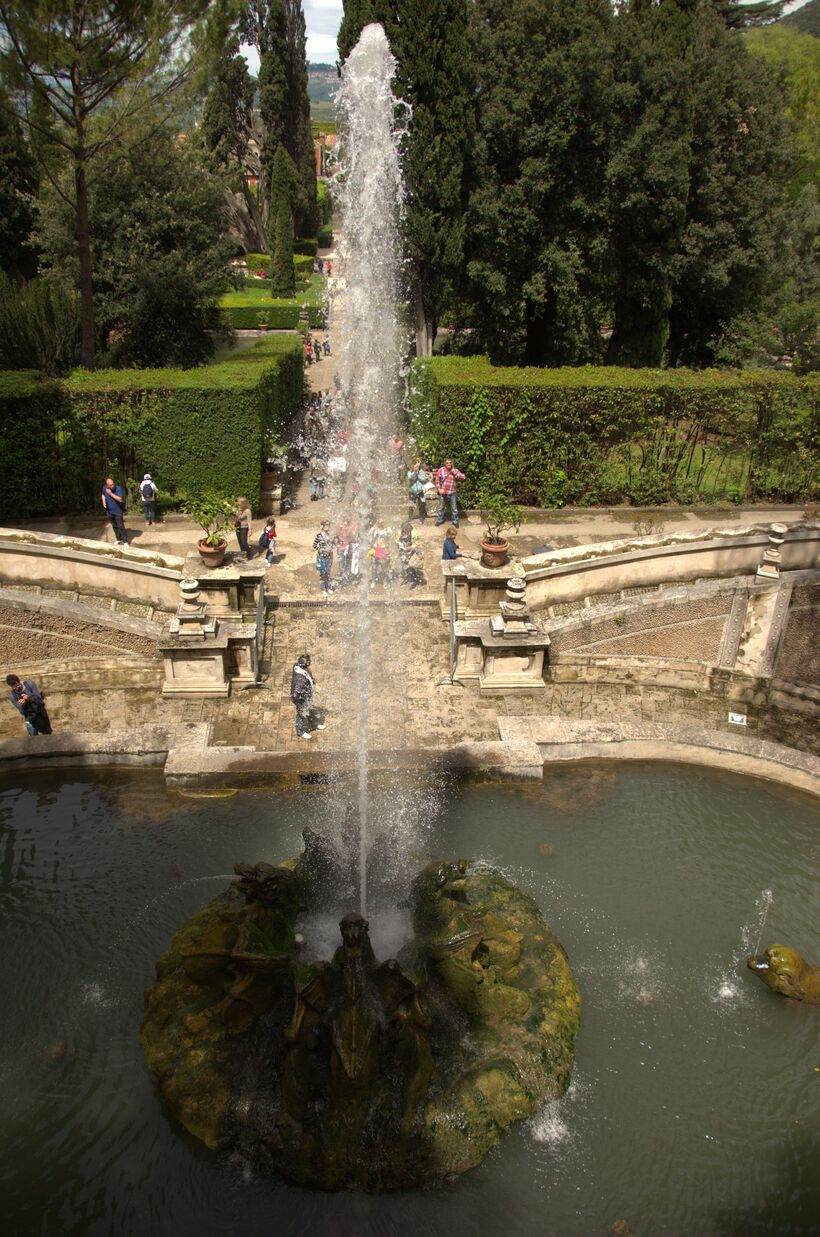
\includegraphics[height=\linewidth]{images/original/r002fc3e2t.jpeg}
    \caption{r002fc3e2t}
    \end{subfigure}\hfill%
    \begin{subfigure}[c]{.31\linewidth}\centering
    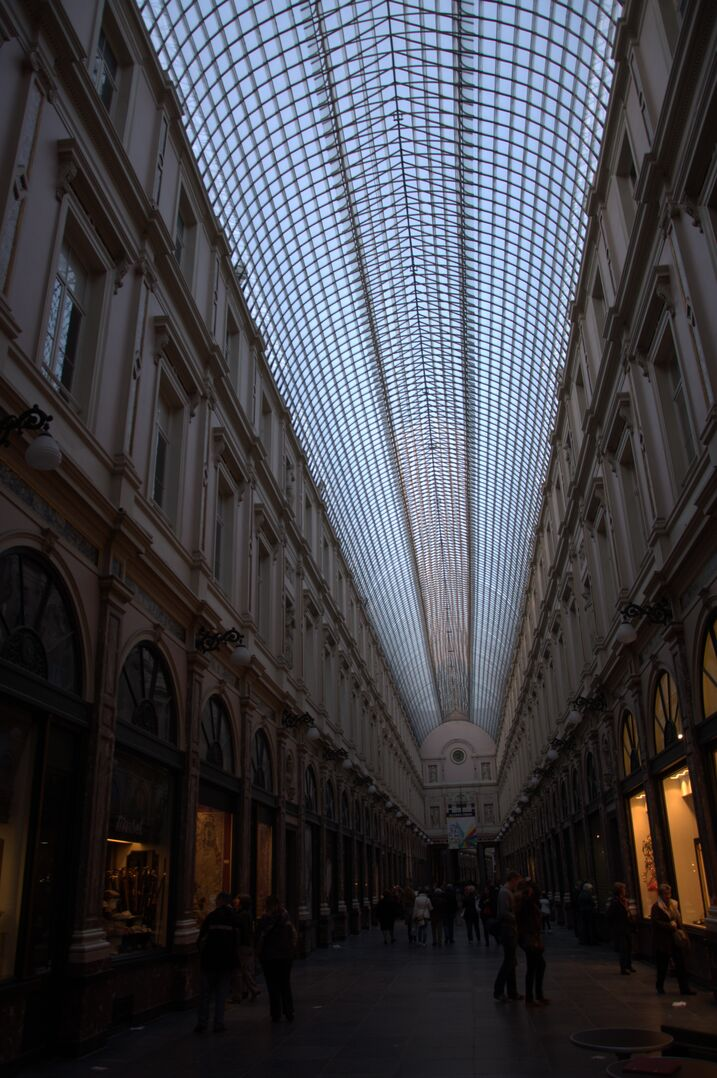
\includegraphics[height=\linewidth]{images/original/r1ead3024t.jpeg}
    \caption{r1ead3024t}
    \end{subfigure}\hfill%
    \begin{subfigure}[c]{.31\linewidth}\centering
    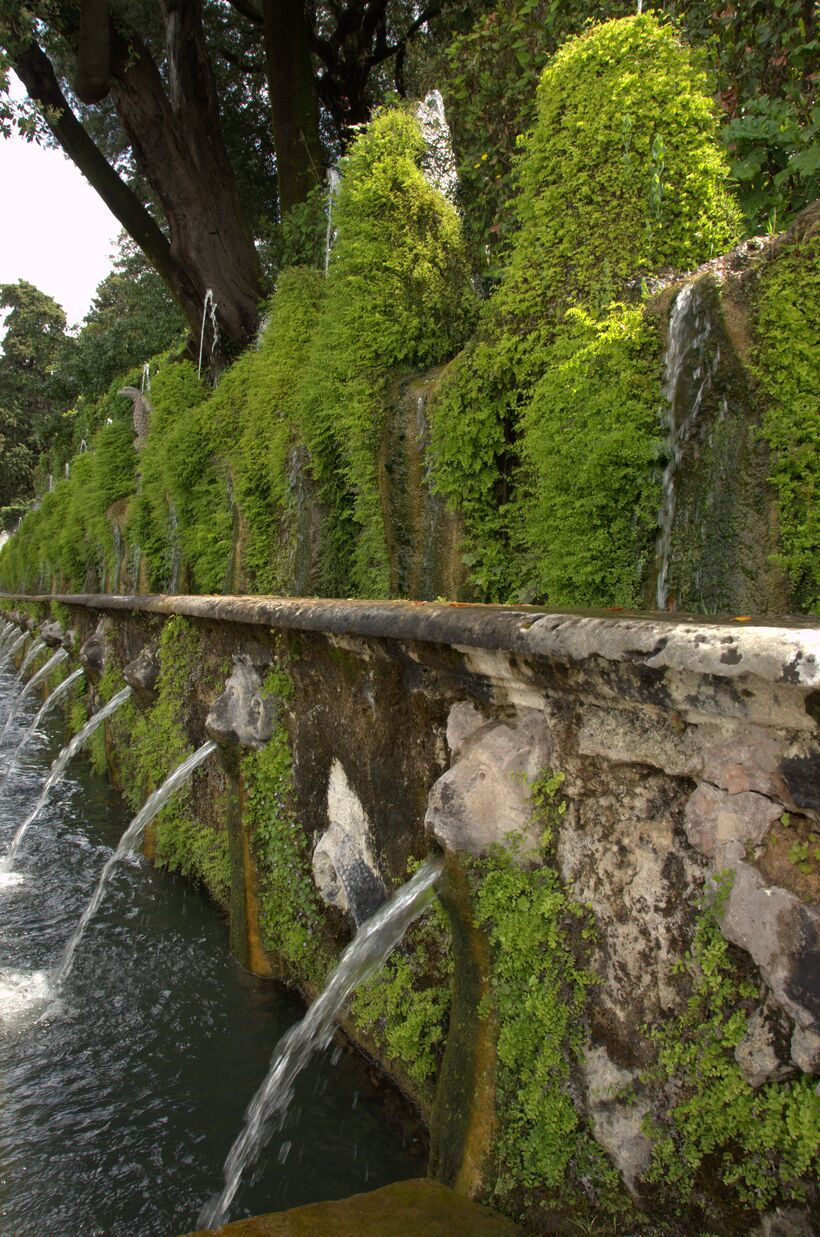
\includegraphics[height=\linewidth]{images/original/r1ceba29dt.jpeg}
    \caption{r1ceba29dt}
    \end{subfigure}%
    
    \begin{subfigure}[c]{.31\linewidth}\centering
    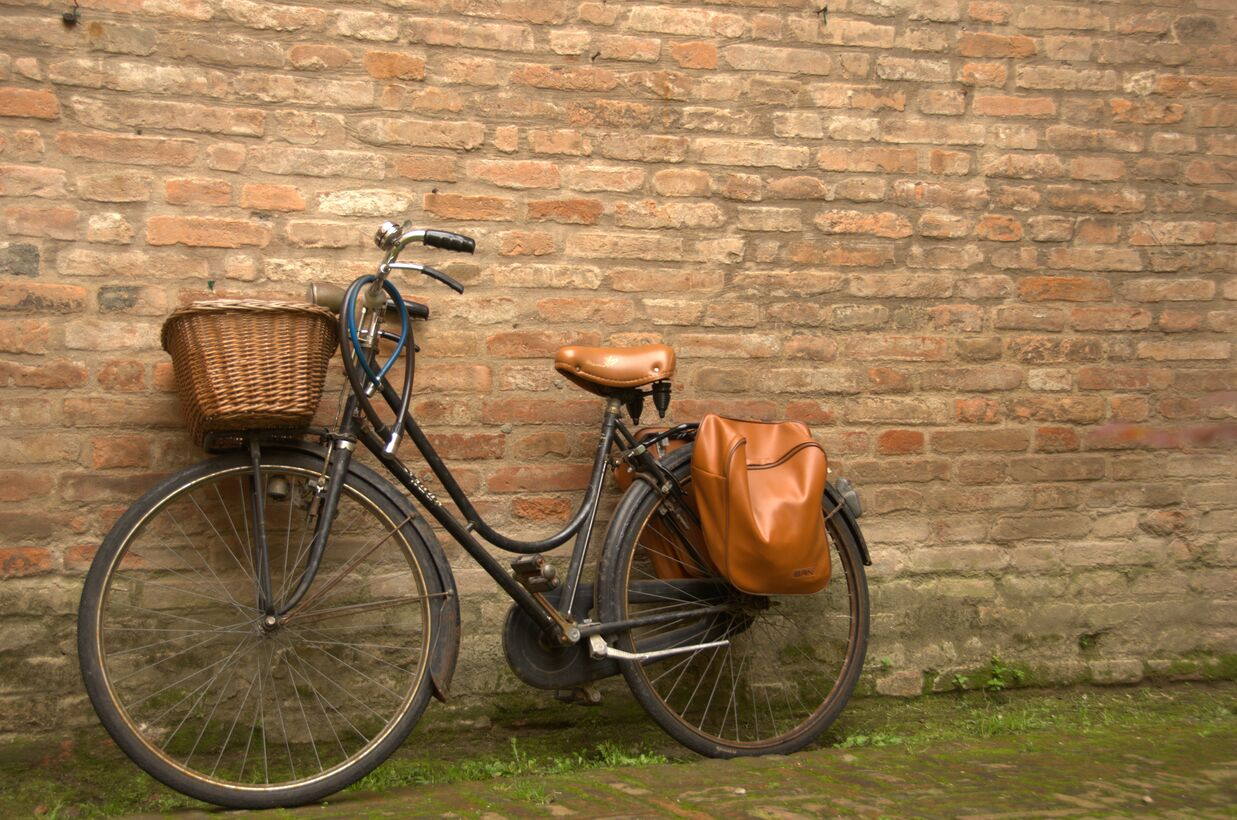
\includegraphics[width=\linewidth]{images/original/r0a2ff882t.jpeg}
    \caption{r0a2ff882t}
    \end{subfigure}\hfill%
    \begin{subfigure}[c]{.31\linewidth}\centering
    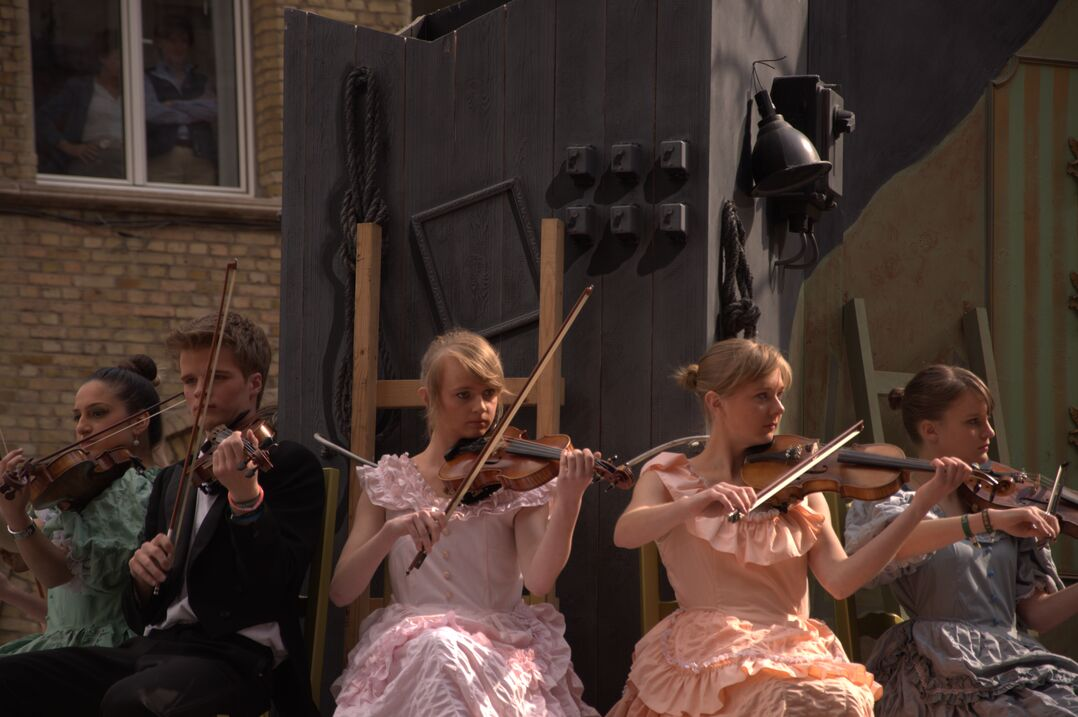
\includegraphics[width=\linewidth]{images/original/r0a808003t.jpeg}
    \caption{r0a808003t}
    \end{subfigure}\hfill%
    \begin{subfigure}[c]{.31\linewidth}\centering
    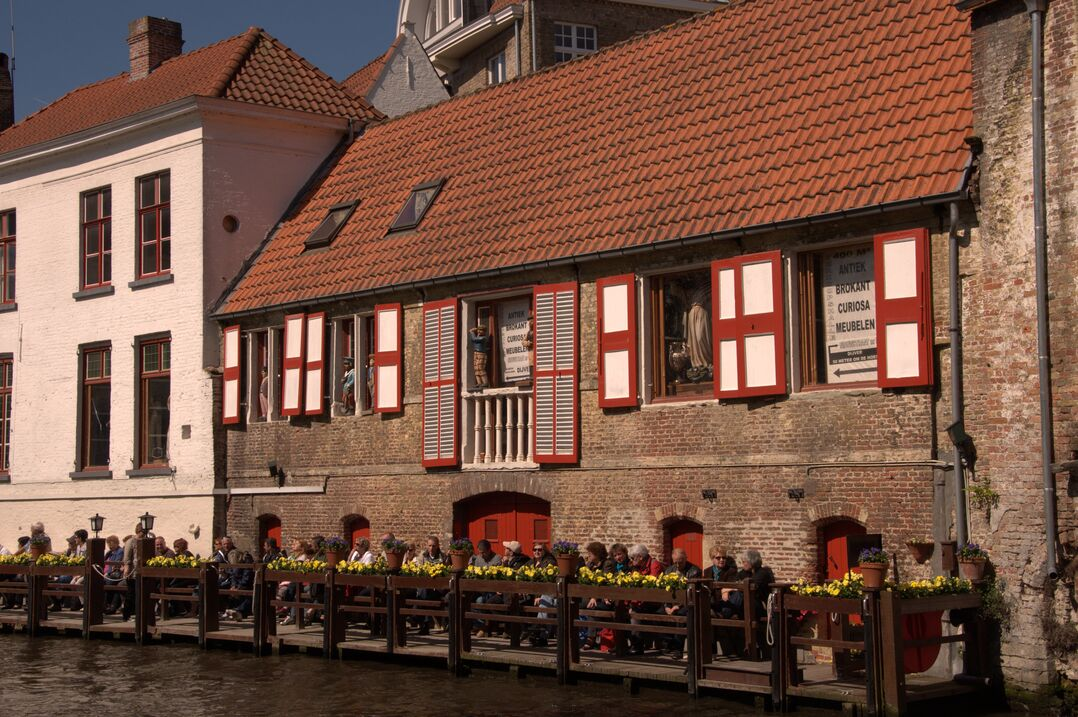
\includegraphics[width=\linewidth]{images/original/r0a966704t.jpeg}
    \caption{r0a966704t}
    \end{subfigure}
    
    \begin{subfigure}[c]{.31\linewidth}\centering
    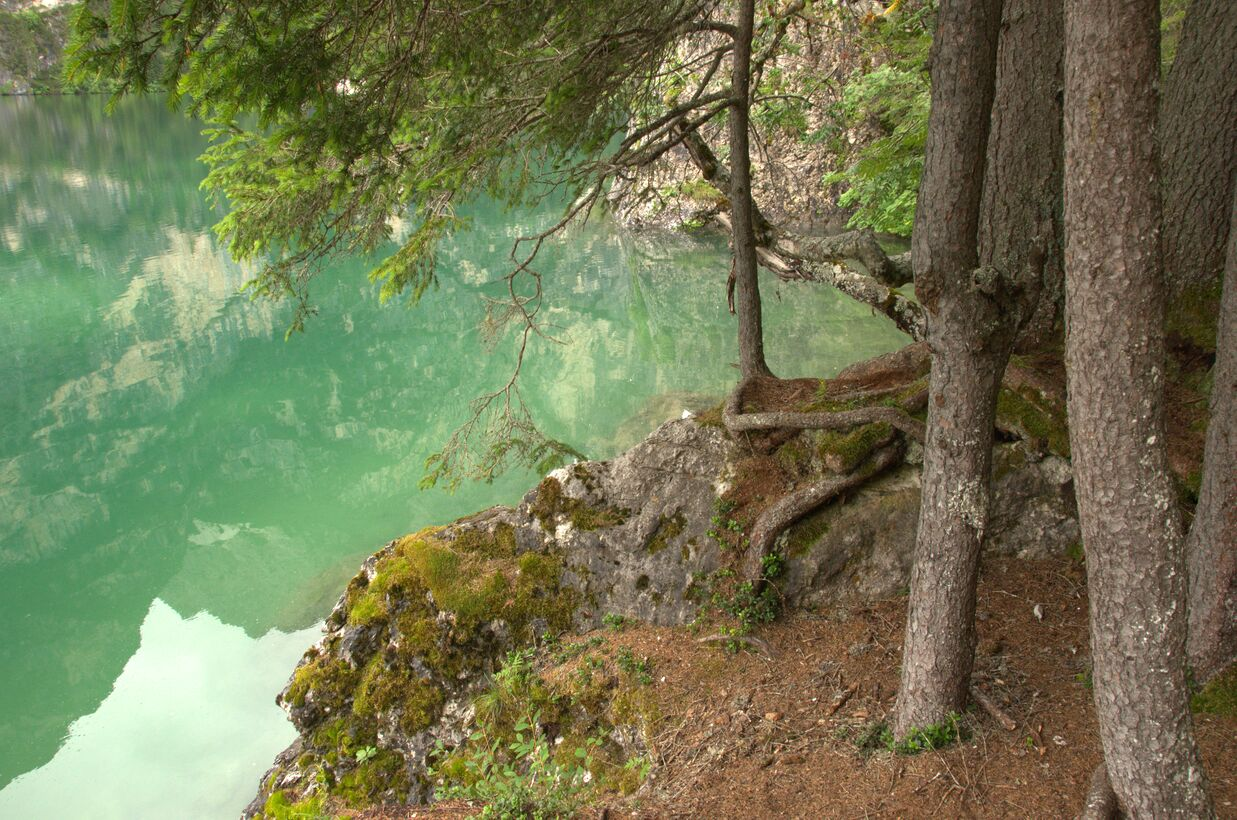
\includegraphics[width=\linewidth]{images/original/r0e04cc91t.jpeg}
    \caption{r0e04cc91t}
    \end{subfigure}\hfill%
    \begin{subfigure}[c]{.31\linewidth}\centering
    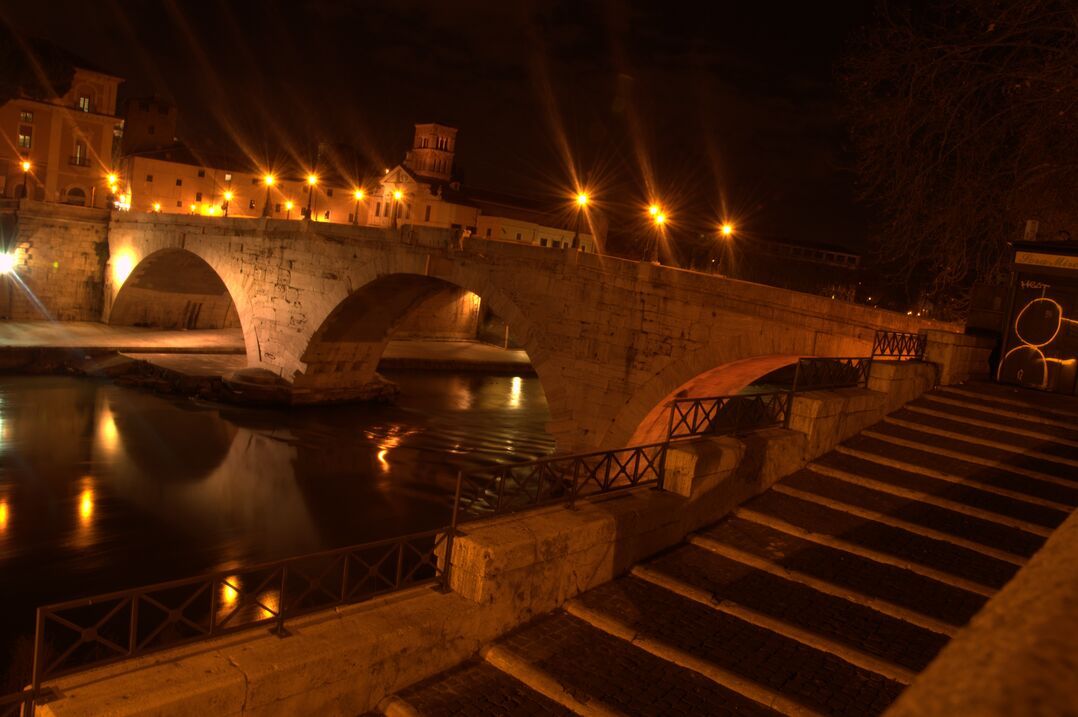
\includegraphics[width=\linewidth]{images/original/r0ea0825ft.jpeg}
    \caption{r0ea0825ft}
    \end{subfigure}\hfill%
    \begin{subfigure}[c]{.31\linewidth}\centering
    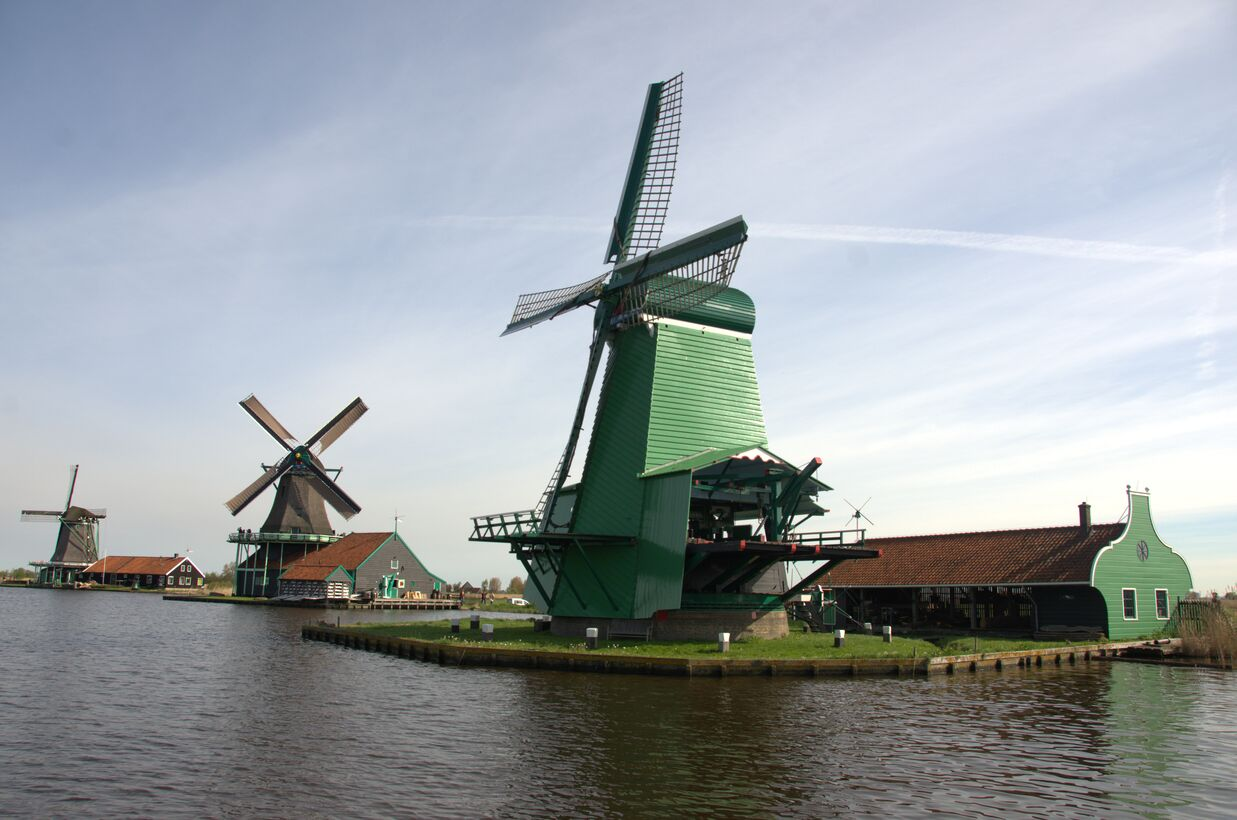
\includegraphics[width=\linewidth]{images/original/r1a0f5585t.jpeg}
    \caption{r1a0f5585t}
    \end{subfigure}
    
    \begin{subfigure}[c]{.31\linewidth}\centering
    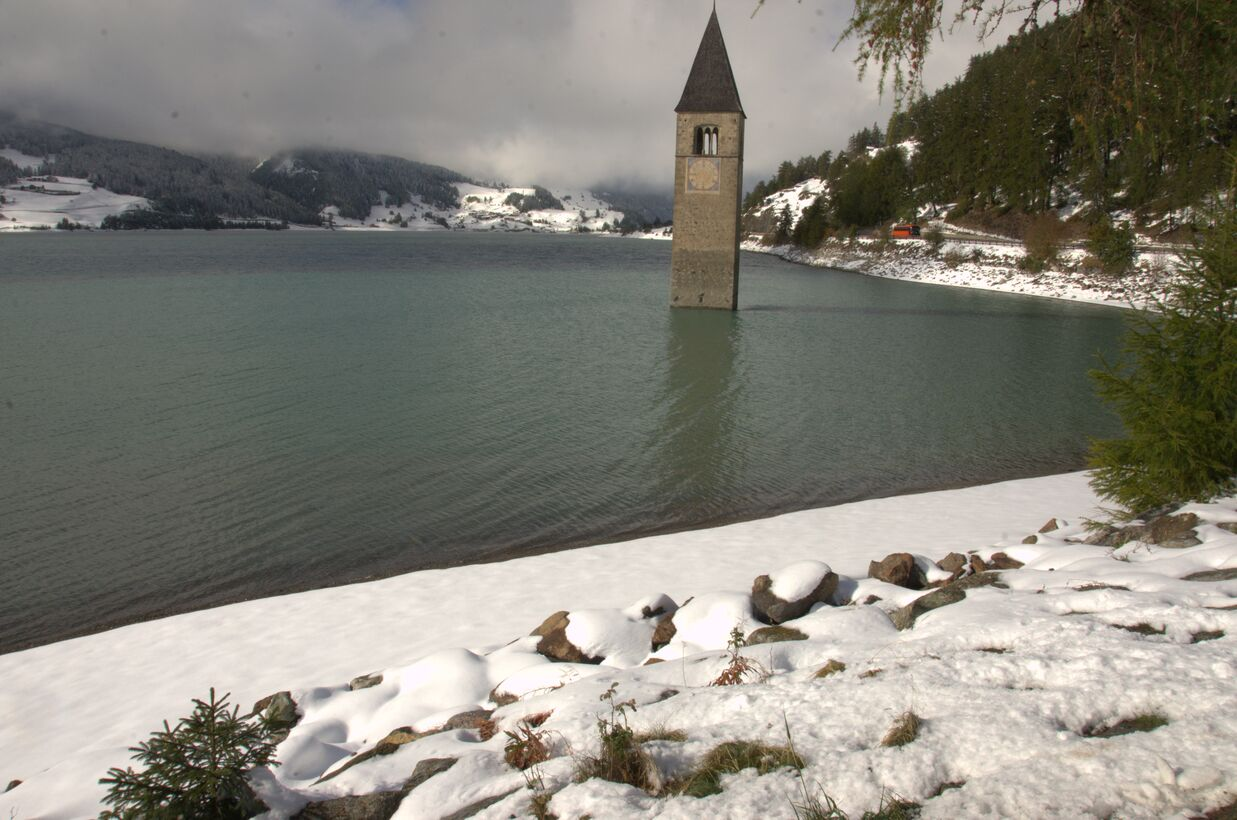
\includegraphics[width=\linewidth]{images/original/r1c9fdcf4t.jpeg}
    \caption{r1c9fdcf4t}
    \end{subfigure}\hfill%
    \begin{subfigure}[c]{.31\linewidth}\centering
    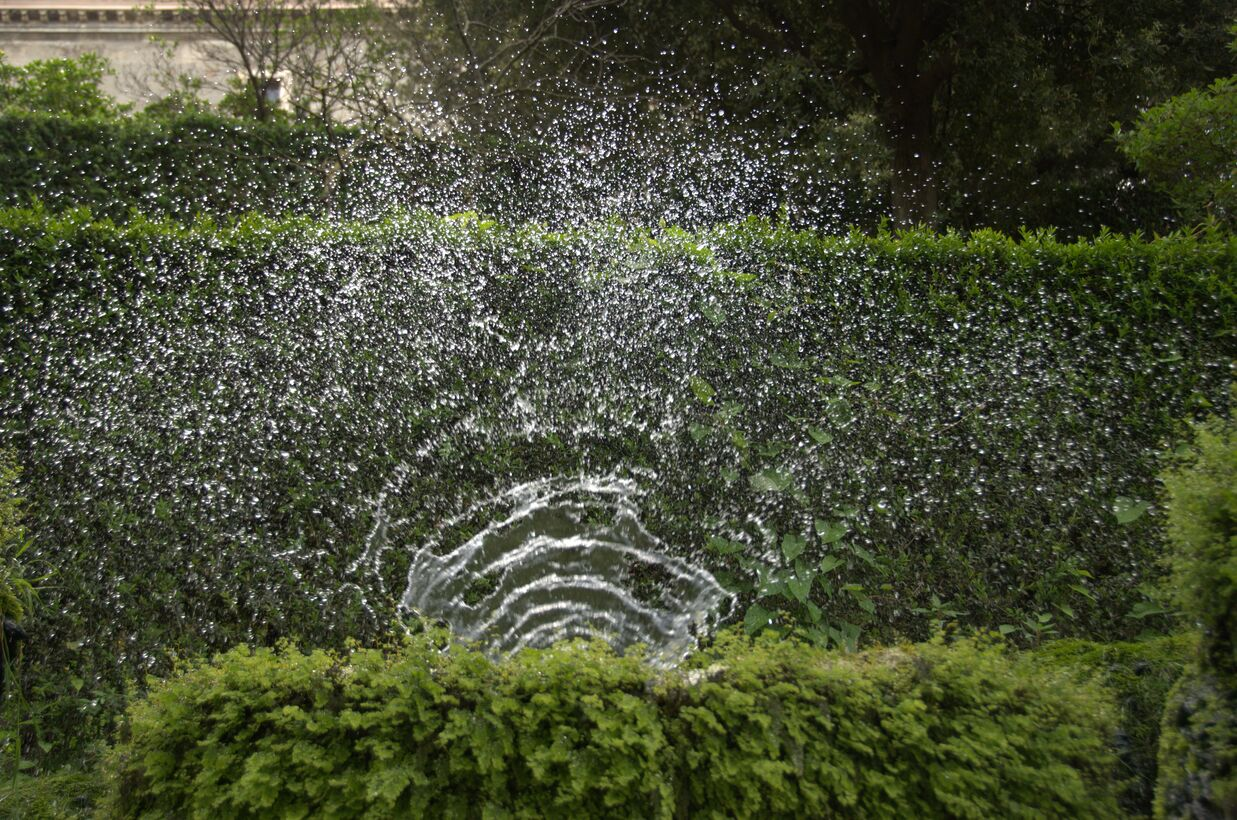
\includegraphics[width=\linewidth]{images/original/r06aa7dabt.jpeg}
    \caption{r06aa7dabt}
    \end{subfigure}\hfill%
    \begin{subfigure}[c]{.31\linewidth}\centering
    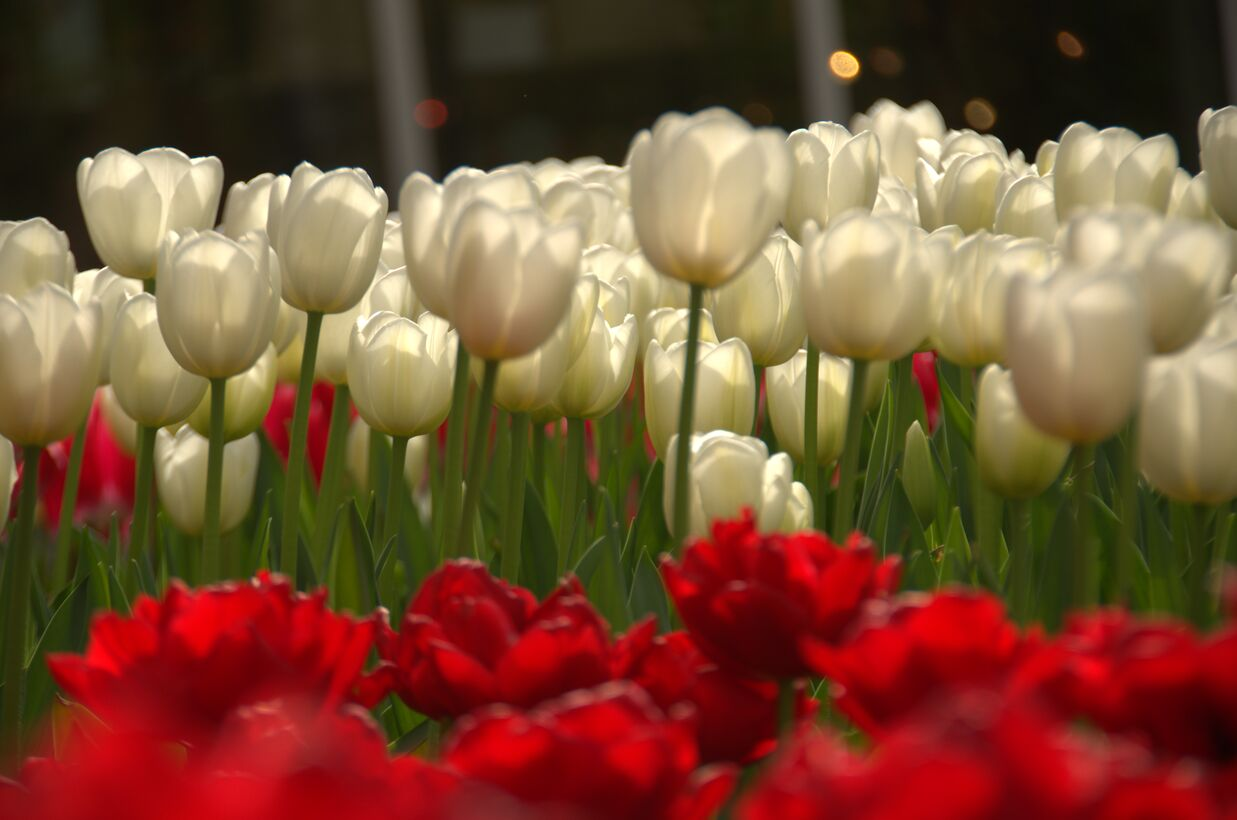
\includegraphics[width=\linewidth]{images/original/r07cfb432t.jpeg}
    \caption{r07cfb432t}
    \end{subfigure}
    
    \begin{subfigure}[c]{.31\linewidth}\centering
    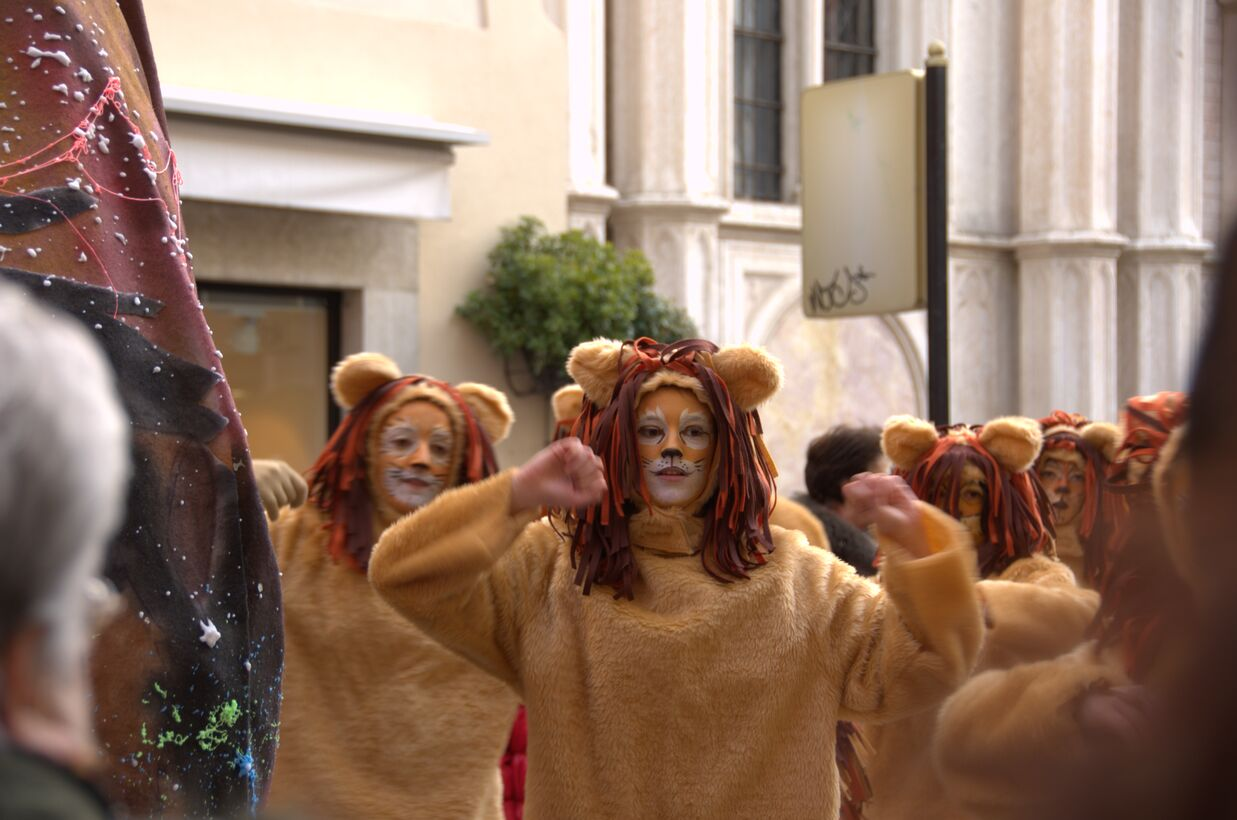
\includegraphics[width=\linewidth]{images/original/r07ffdc87t.jpeg}
    \caption{r07ffdc87t}
    \end{subfigure}\hfill%
    \begin{subfigure}[c]{.31\linewidth}\centering
    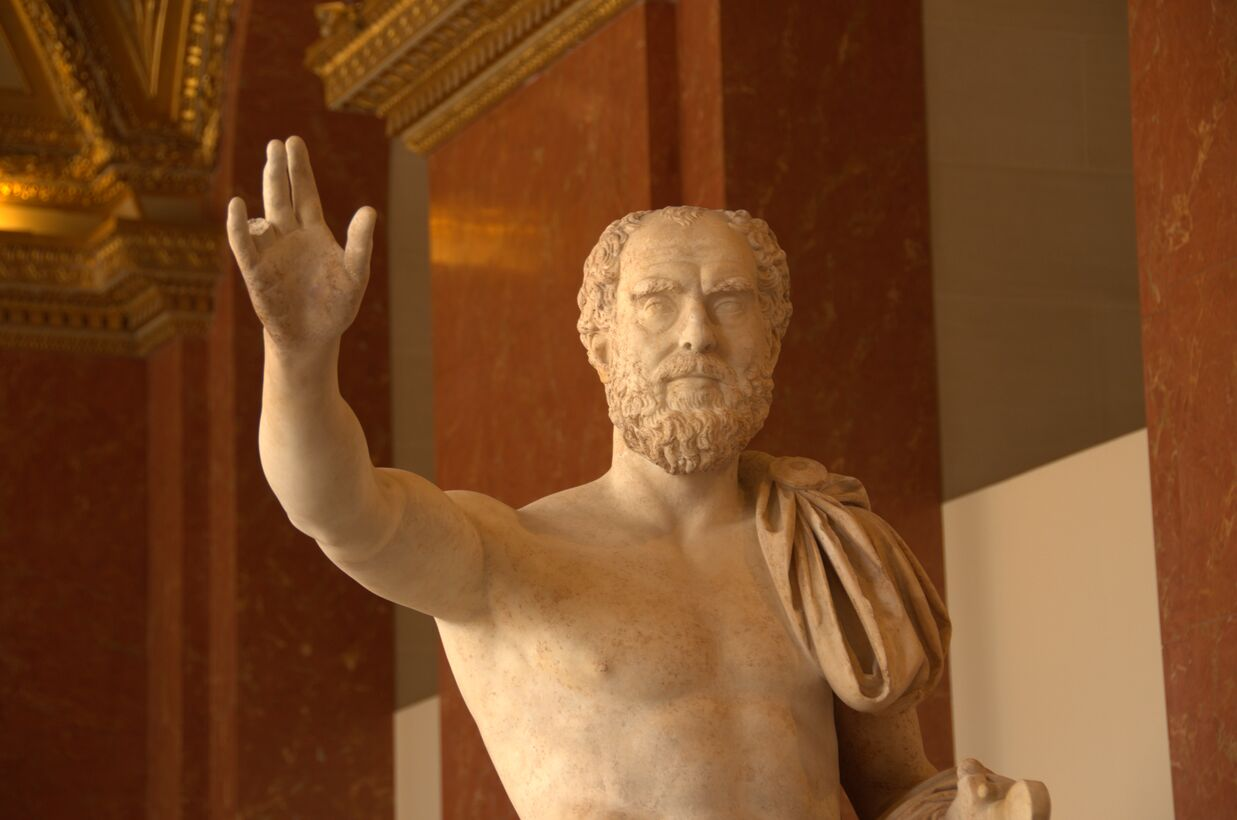
\includegraphics[width=\linewidth]{images/original/r16da5576t.jpeg}
    \caption{r16da5576t}
    \end{subfigure}\hfill%
    \begin{subfigure}[c]{.31\linewidth}\centering
    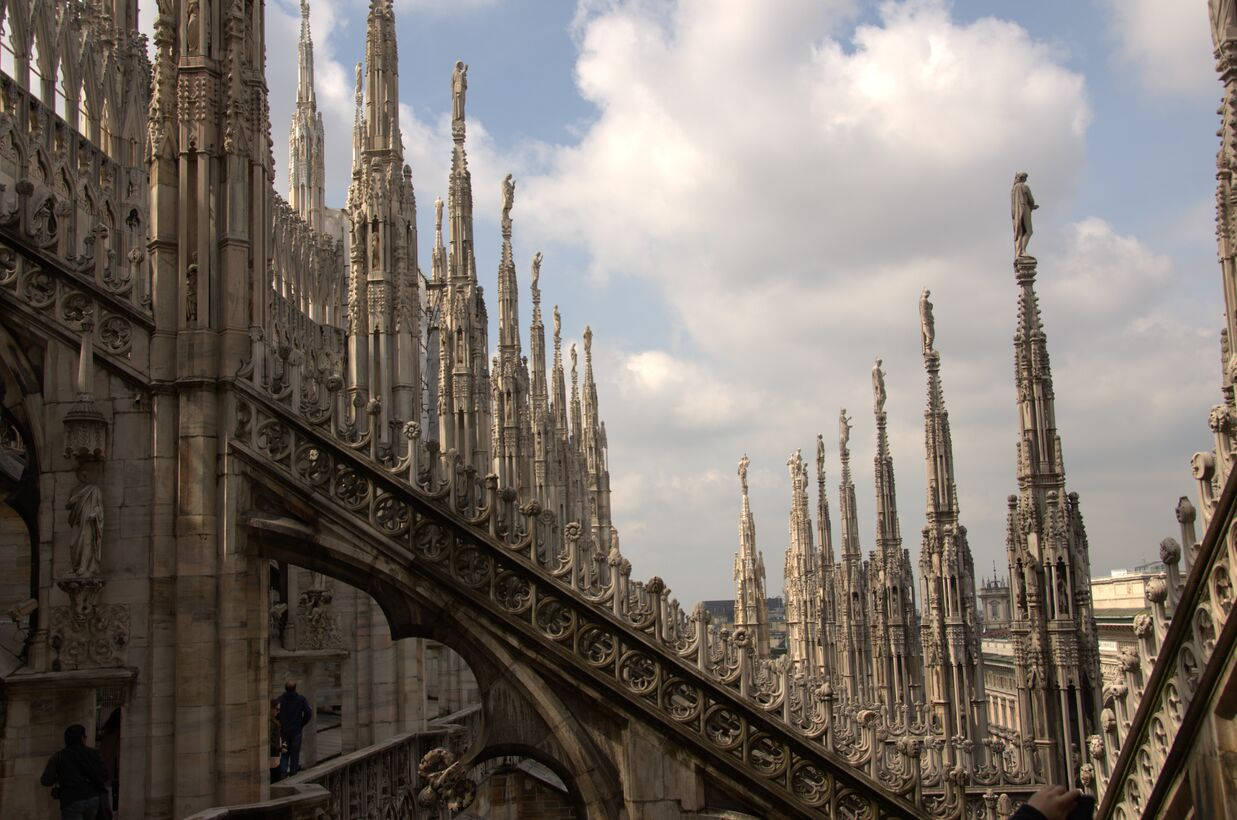
\includegraphics[width=\linewidth]{images/original/r191f3cdet.jpeg}
    \caption{r191f3cdet}
    \end{subfigure}
    
    \caption{Those 15 images from the Raise Dataset~\cite{raise} were used during our experiments.}
    \label{fig:15images}
\end{figure}

\subsection{CFA pattern detection}
We start by analyzing, at a global scale, whether the method is able to detect the correct pattern of the 15 images described above. Results can be seen in Table~\ref{tab:global}. One can see that the algorithms detects the correct grid in all 15 images when they are demosaiced with bilinear, AHD or DCB demosaicing. It also works very well on the PPG and VNG algorithms, despite a few mistakes in the full pattern identification against PPG or VNG-demosaiced images, which are solved when using bidirectional filters. When the image is demosaiced with AAHD or DHT, however, the algorithm consistently fails to detect even the diagonal, and consequently also fails on the full pattern, in both versions of the algorithm.
\begin{table}[ht]
    \centering
        \begin{subfigure}[t]{.5\linewidth}
                \centering
    \begin{tabular}{lcc}
    \toprule
    Demosaicking & Diagonal & Full pattern\\
    \midrule
    AAHD & \color{c2}0/15 & \color{c2}0/15\\
    AHD & \color{c0}15/15 & \color{c0}15/15\\
    DCB & \color{c0}15/15 & \color{c0}15/15\\
    DHT & \color{c2}3/15 & \color{c2}3/15\\
    Bilinear & \color{c0}15/15 & \color{c0}15/15\\
    PPG & \color{c0}15/15 & \color{c3}13/15\\
    VNG & \color{c0}15/15 & \color{c3}14/15\\
    \bottomrule
    \end{tabular}
                \caption{Original isotropic intermediate values computation}
        \end{subfigure}\hfill%
        \begin{subfigure}[t]{.5\linewidth}
                \centering
    \begin{tabular}{lcc}
    \toprule
    Demosaicking & Diagonal & Full pattern\\
    \midrule
    AAHD & \color{c2}0/15 & \color{c2}0/15\\
    AHD & \color{c0}15/15 & \color{c0}15/15\\
    DCB & \color{c0}15/15 & \color{c0}15/15\\
    DHT & \color{c2}2/15 & \color{c2}2/15\\
    Bilinear & \color{c0}15/15 & \color{c0}15/15\\
    PPG & \color{c0}15/15 & \color{c0}15/15\\
    VNG & \color{c0}15/15 & \color{c0}15/15\\
    \bottomrule
    \end{tabular}
                \caption{Bidirectional filters for intermediate values computation}
        \end{subfigure}\hfill%
    \label{tab:global}
    \caption{Identification of the main diagonal and of the full pattern on the 15 images. In its original version, algorithm works very well when the demosaicing is done with AHD, DCB or Bilinear demosaicing, with a few errors on the full pattern against PPG- or VNG-demosaiced images. It fails to detect even the diagonal on AAHD- and DHT-demosaiced images. Bidirectional filters for intermediate value computation yields perfect results on PPG and VNG, but still fails against AAHD- and DHT-demosaiced images.}
\end{table}

Looking at the results on image r0a2ff882t, on Figure~\ref{fig:bike}, we can see again that the results are dependant on the demosaicing algorithm used by the method. All windows are detected correctly against DCB and Bilinear demosicing, but the algorithm is confused on the diagonal pattern in the PPG-demosaiced image, though bidirectional filters for the intermediate value computation partly alleviate this problem. on the VNG-demosaiced image, there are also false detections on the diagonal itself. More importantly, the basket of the bike causes errors with AHD, PPG and VNG demosaicing. This is to be expected, as this is a textured region, but could easily be misinterpreted as a forgery.
As can be seen on Figure~\ref{fig:bike_ahd}, however, using bidirectional filters yields a very low relative confidence for the identification of the basket's grid compared to the rest of the image. As a consequence, a reasonable thresholding level should still enable one to automatically discard this false detection.

\def\s{.12\linewidth}
\setlength{\tabcolsep}{0.2em}
\begin{figure}[ht]
        \centering
        \begin{tabular}{cccccccc}
                \multicolumn{8}{c}{
                        \begin{tabular}{cl}
                                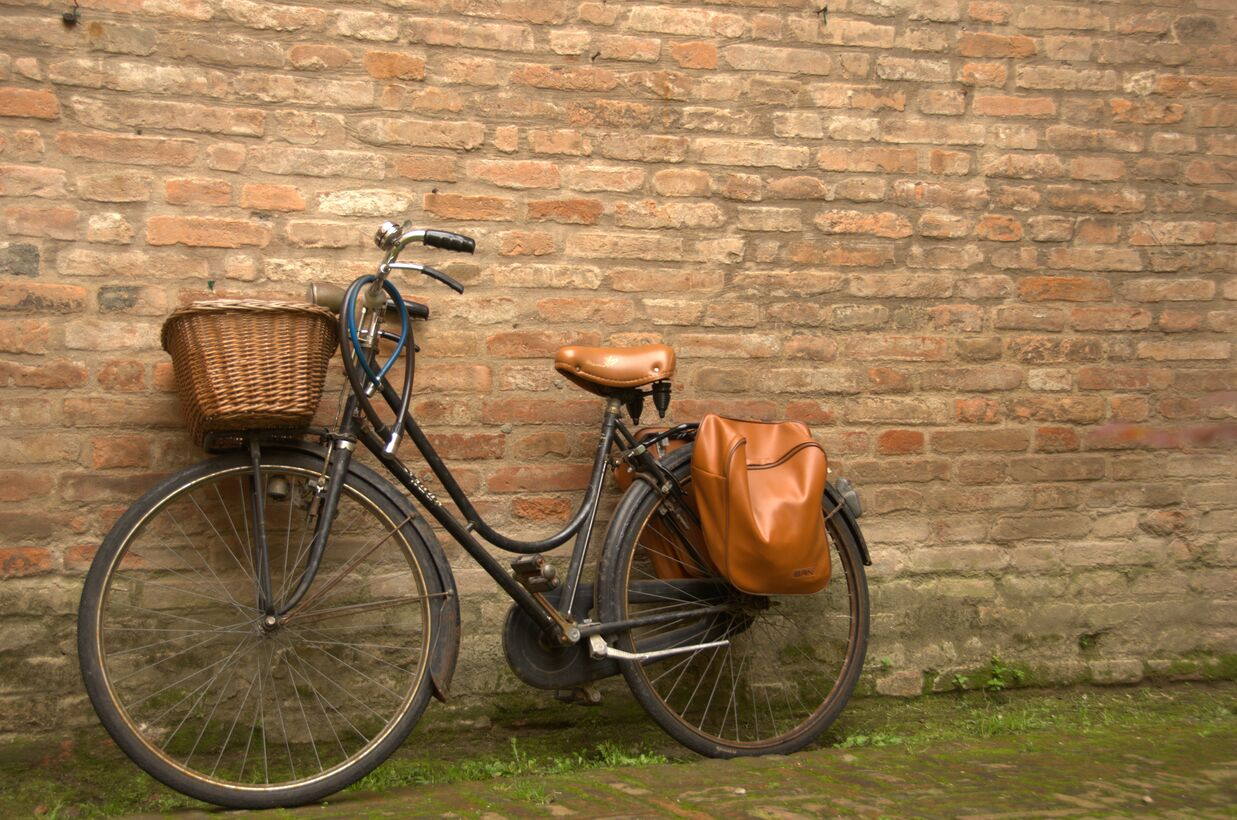
\includegraphics[width=.6\linewidth]{images/original/r0a2ff882t.jpeg}&
                                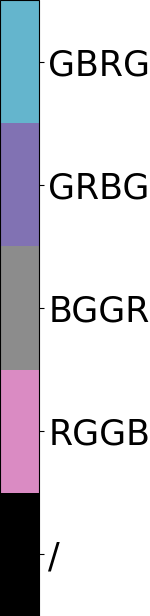
\includegraphics[height=150pt]{images/cb.png}\\
                                Original image (r0a2ff882t), in \textsc{rggb} pattern&
                        \end{tabular}
                }\\                                
                & AAHD & AHD & DCB & DHT & Bilinear & PPG & VNG\\
                \midrule
                \raisebox{5pt}{\rotatebox{90}{\tiny Original}} & 
                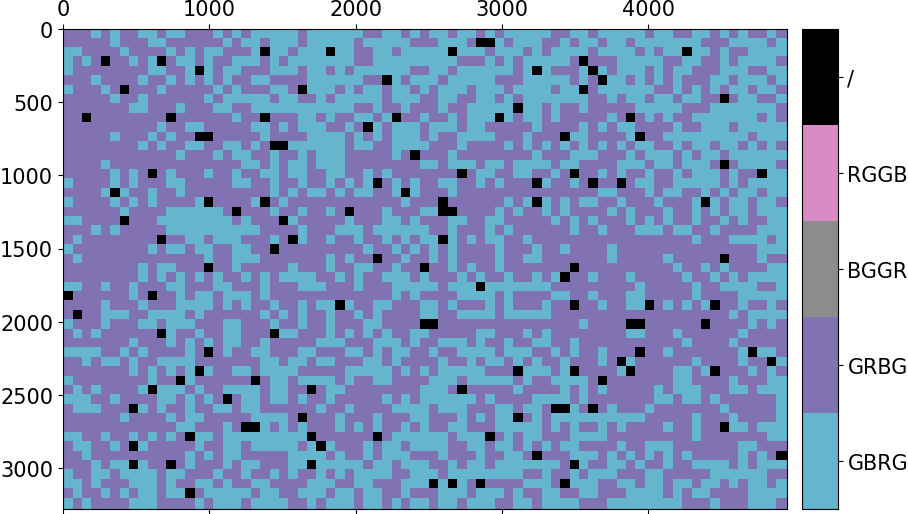
\includegraphics[width=\s]{images/bike/AAHD/iso_64_grids.png} &
                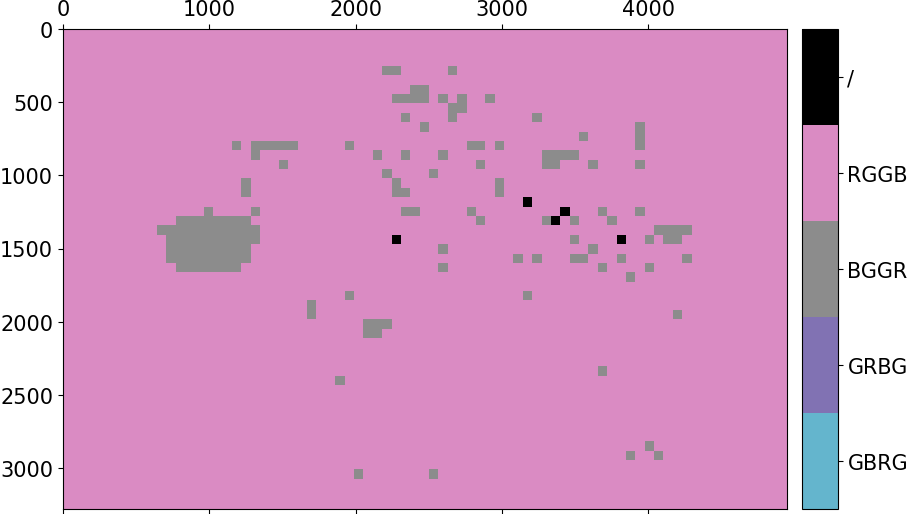
\includegraphics[width=\s]{images/bike/AHD/iso_64_grids.png} &
                
\includegraphics[width=\s]{images/bike/DCB/iso_64_grids.png} &
                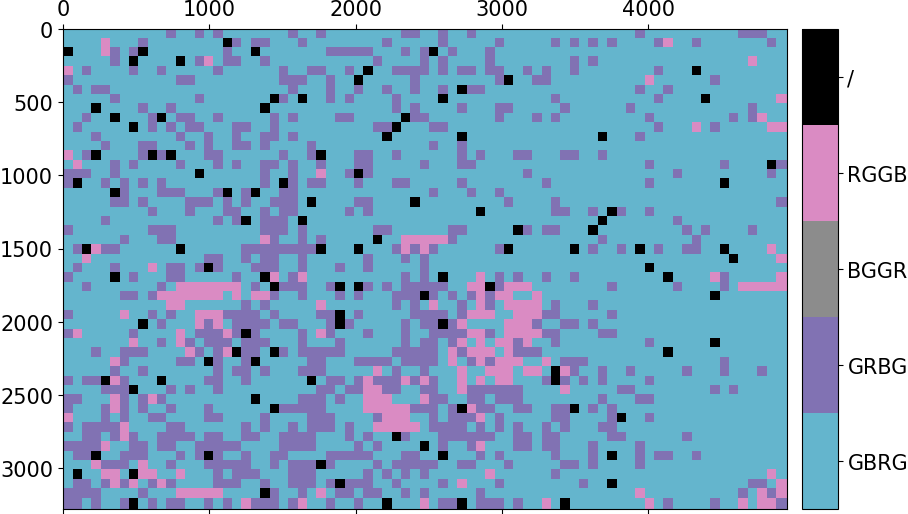
\includegraphics[width=\s]{images/bike/DHT/iso_64_grids.png} &
                
\includegraphics[width=\s]{images/bike/LINEAR/iso_64_grids.png} &
                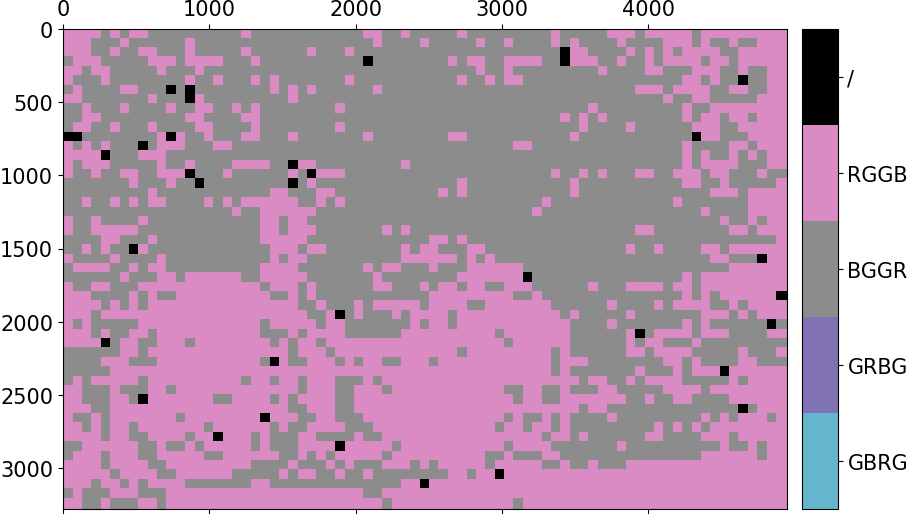
\includegraphics[width=\s]{images/bike/PPG/iso_64_grids.png} &
                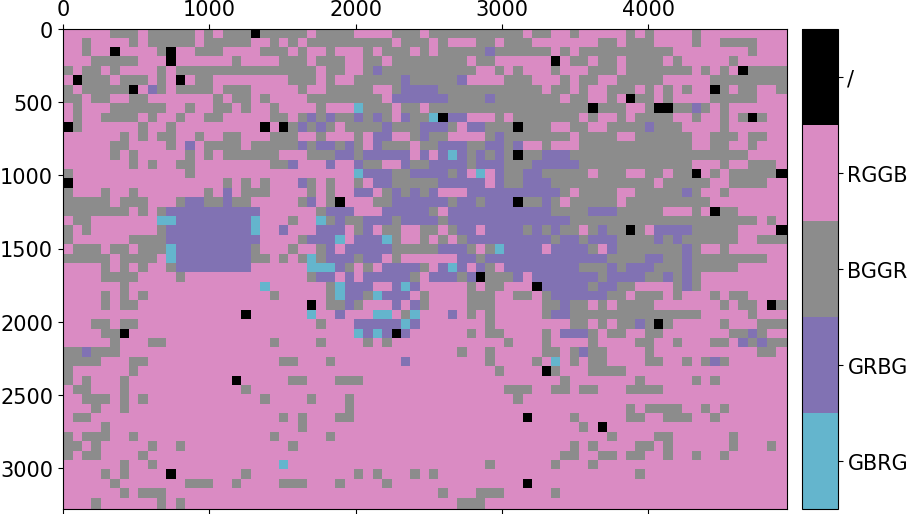
\includegraphics[width=\s]{images/bike/VNG/iso_64_grids.png} \\
                \rotatebox{90}{\tiny Bidirectional} & 
                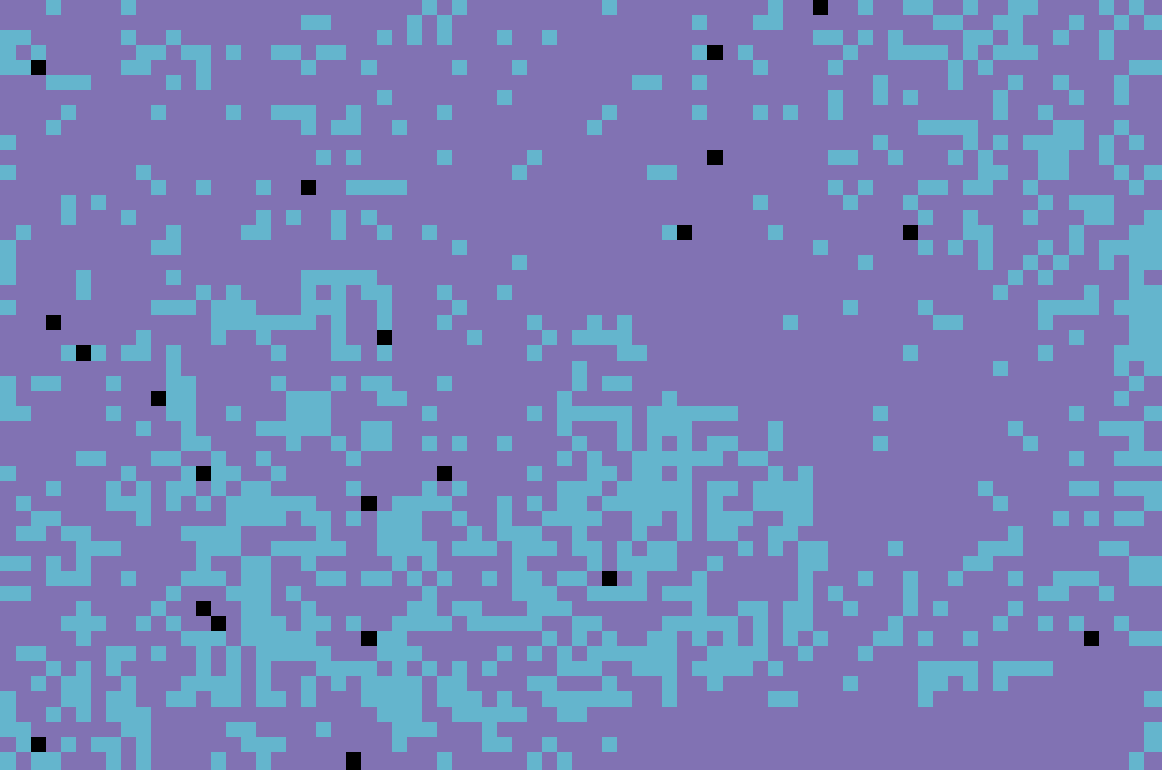
\includegraphics[width=\s]{images/bike/AAHD/bid_64_grids.png} &
                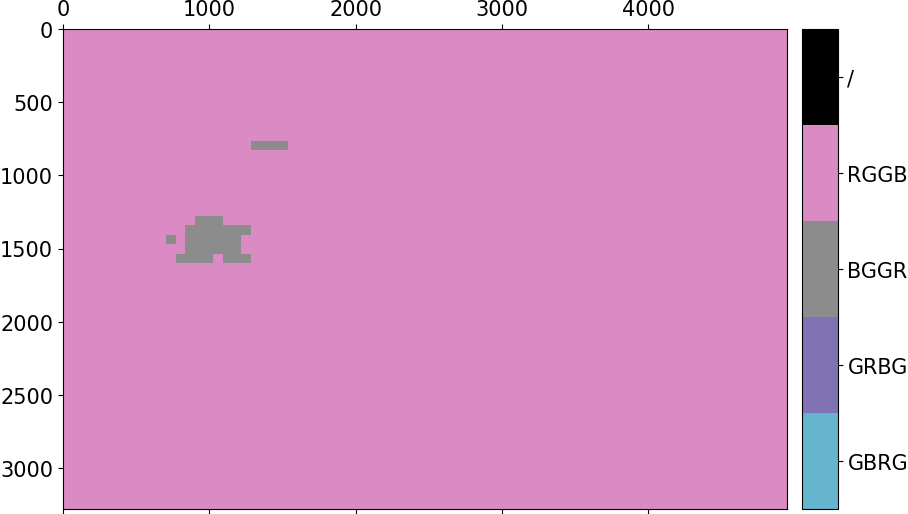
\includegraphics[width=\s]{images/bike/AHD/bid_64_grids.png} &
                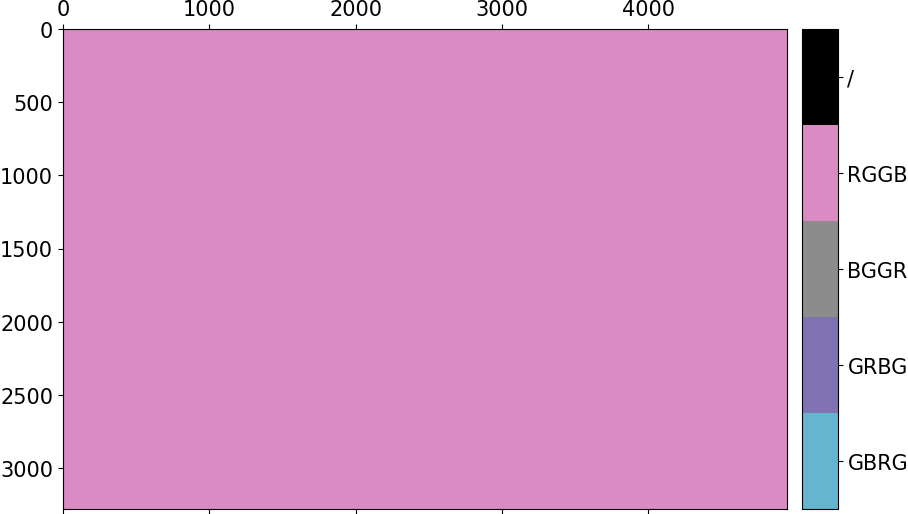
\includegraphics[width=\s]{images/bike/DCB/bid_64_grids.png} &
                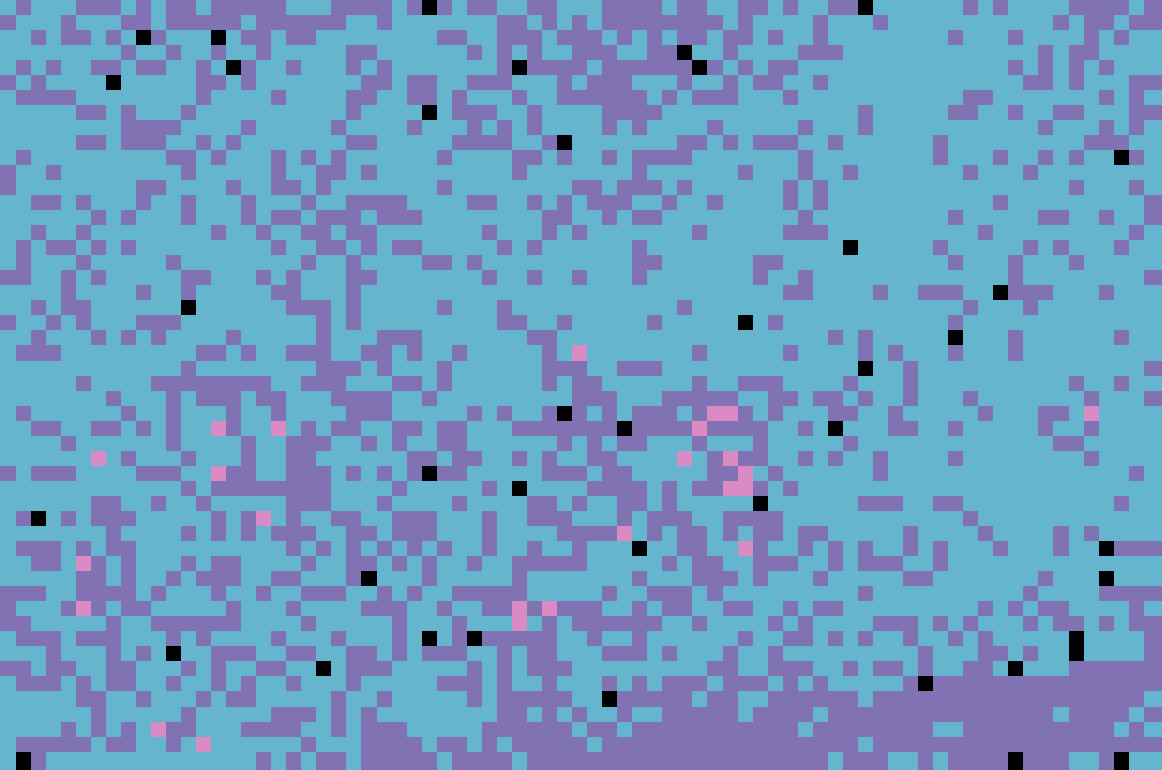
\includegraphics[width=\s]{images/bike/DHT/bid_64_grids.png} &
                
\includegraphics[width=\s]{images/bike/LINEAR/bid_64_grids.png} &
                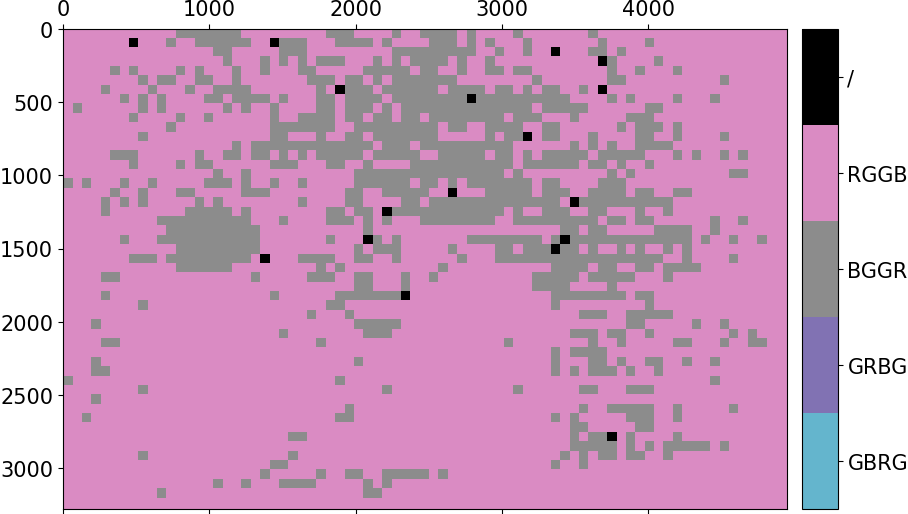
\includegraphics[width=\s]{images/bike/PPG/bid_64_grids.png} &
                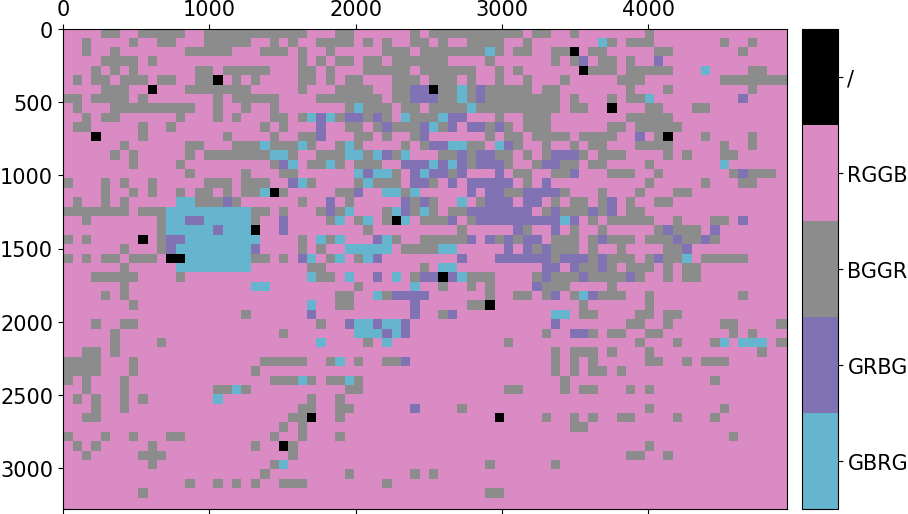
\includegraphics[width=\s]{images/bike/VNG/bid_64_grids.png}\\
                \bottomrule
        \end{tabular}
\caption{Results of the method on 64×64 windows, both with the original isotropic intermediate value mask and the proposed bidirectional one, on one image with the 7 different demosaicing algorithms. Both method work perfectly on the DCB- and Bilinear-demosaiced images. With the AHD, PPG and VNG methods, both methods have trouble discerning between the two patterns sharing the same diagonal, but the bidirectional detection makes fewer mistakes. Textured regions such as the basket can create a localized shift in the detected mosaic, which could be interpretated as a forgery.
With the AAHD and DHT algorithm, the method consistently detects the wrong diagonal.}
\label{fig:bike}
\end{figure}



\begin{figure}[ht]
\centering
\begin{subfigure}[t]{.5\linewidth}
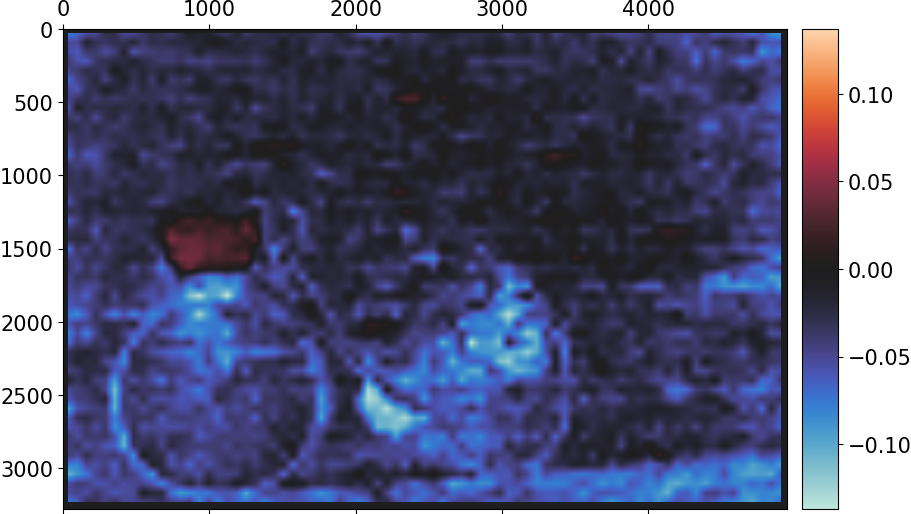
\includegraphics[width=\linewidth]{images/bike/ahd_iso_64_diff_rggb_bggr.png}
\caption{Isotropic}
\end{subfigure}%
\begin{subfigure}[t]{.5\linewidth}
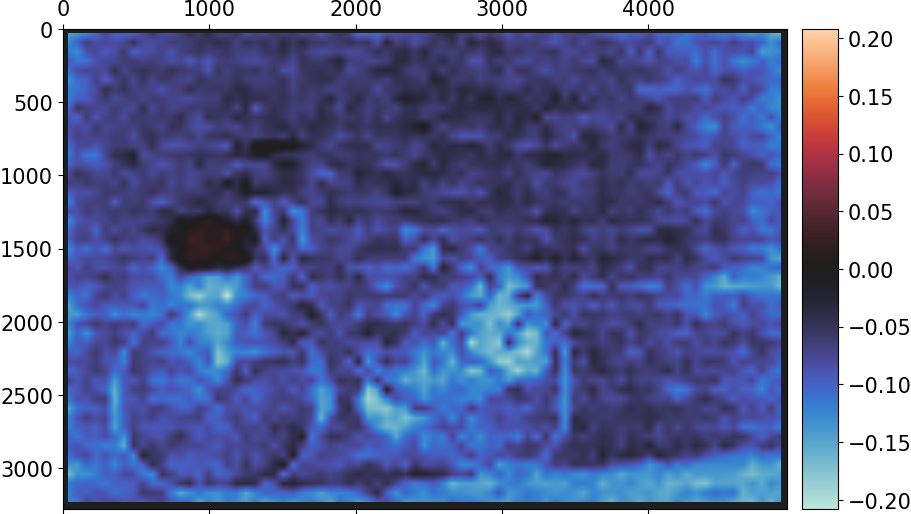
\includegraphics[width=\linewidth]{images/bike/ahd_bid_64_diff_rggb_bggr.png}
\caption{Bidirectional}
\end{subfigure}
        \label{fig:bike_ahd}
\caption{This figure shows, on the AHD-demosaiced bicycle image, the difference of counts of intermediate values corresponding to the \textsc{rggb} and \textsc{bggr} patterns, on the red and blue channels. This count is what is used by the algorithm to decide on a grid. A negative difference corresponds to the correct \textsc{rggb} pattern, a positive difference to the incorrect \textsc{bggr} pattern. The difference is normalized by dividing it by the size of the block ($64\times64$). The textures in the basket area leads to a locally consistent shift in the position of the intermediate values. The error is slightly less prominent when a bidirectional mask is used, but is still consistently in favour of the wrong grid.}
\end{figure}

Most images that are found on the web are JPEG-compressed. It is thus vital to test the robustness of this algorithm to JPEG compression. JPEG compression quickly discards the highest frequencies, at which CFA artefacts are located. As a consequence, it would be illusory to expect results on heavily-compressed images. However, being able to detect the CFA pattern on low-compression images extends the application range of a CFA grid detection method. We show results after JPEG compression on Figure~\ref{fig:jpeg}. On the two studied images, we can see that even the highest-quality compression of 100 causes many errors in the pattern detection, though the algorithm remains largely usable, especially when only looking at the diagonal. At JPEG quality 98, the algorithm no longer detects the correct pattern, except in the easier case of the bilinear demosaicing algorithm. However, it can still detect the diagonal of most windows, albeit with a few errors. Finally, at JPEG quality 95, the algorithm is unable to find anything.

All in all, JPEG compression remains the biggest limitation of this method, and of CFA detection in general. 

\begin{figure}[ht]
        \centering
        \begin{subfigure}[t]{\linewidth}
        \begin{tabular}{ccccccccc}
                \multicolumn{9}{c}{
                        \begin{tabular}{cl}
                                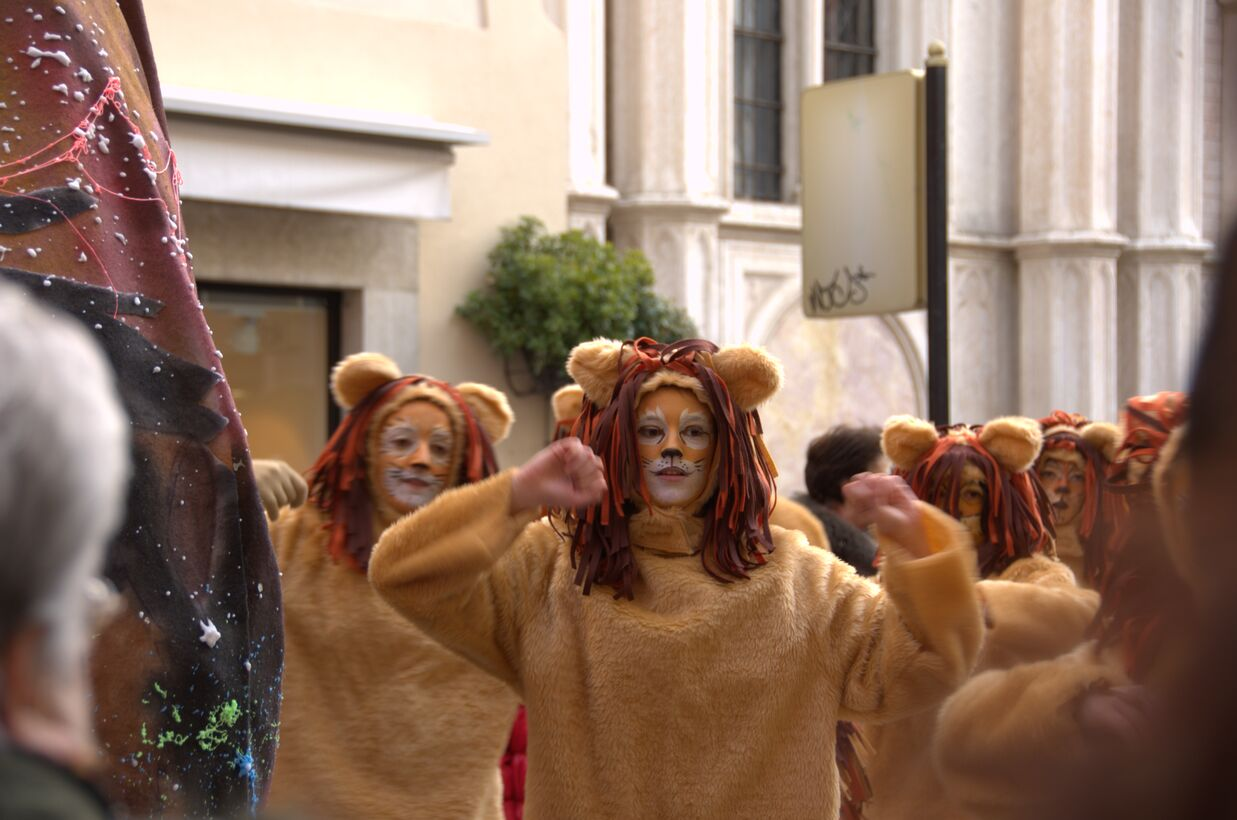
\includegraphics[height=150pt]{images/original/r07ffdc87t.jpeg}&
                                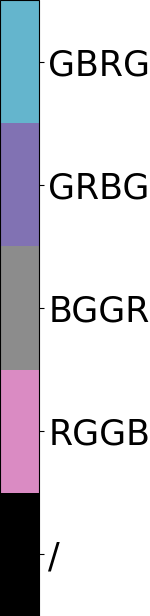
\includegraphics[height=150pt]{images/cb.png}
                        \end{tabular}
                }\\                                
                && AAHD & AHD & DCB & DHT & Bilinear & PPG & VNG\\
                \midrule
                \multirow{2}{*}[1.3em]{{\rotatebox[origin=c]{90}{Uncompressed}}}&
                \raisebox{5pt}{\rotatebox{90}{\tiny Original}} & 
                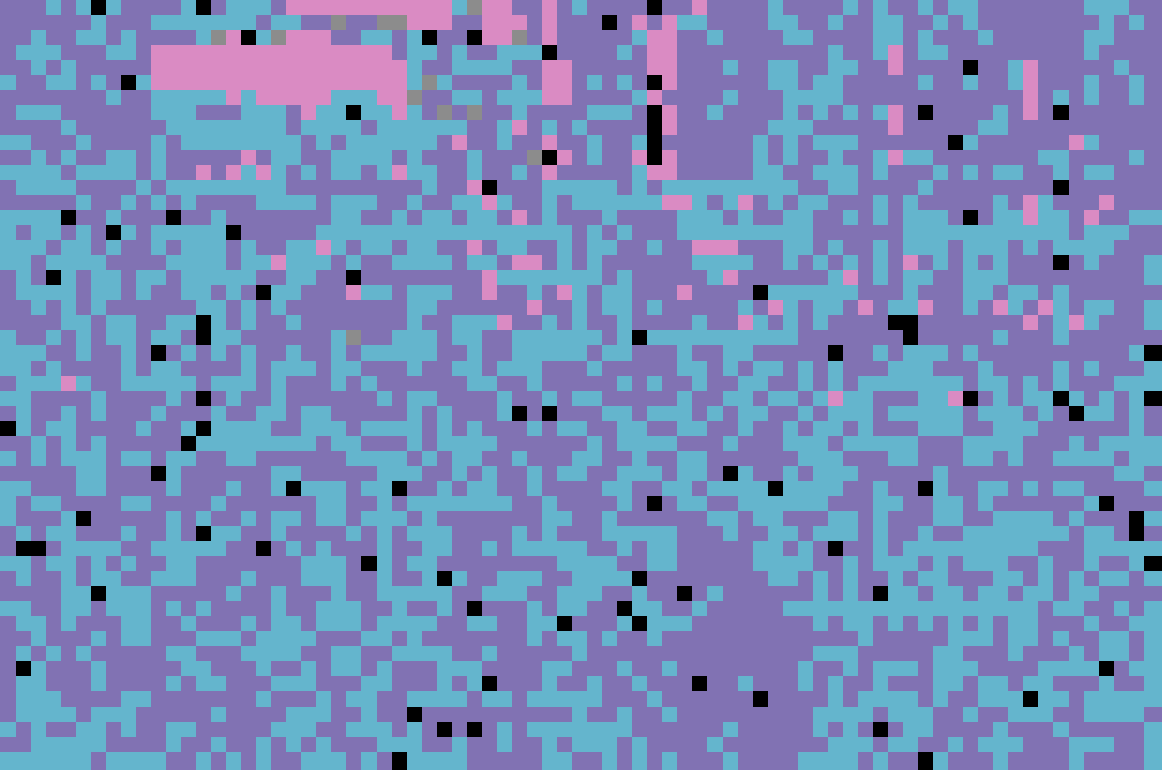
\includegraphics[width=\s]{images/carnival/AAHD/iso_64_grids.png}&
                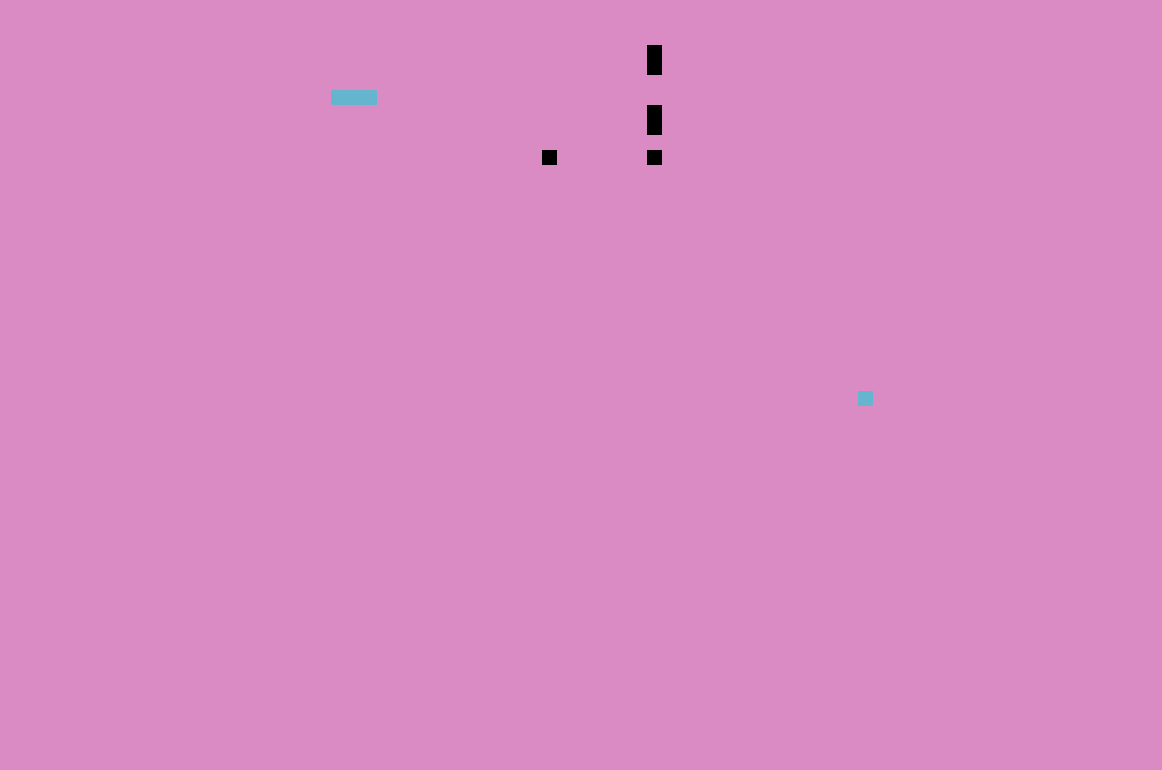
\includegraphics[width=\s]{images/carnival/AHD/iso_64_grids.png}&
                \includegraphics[width=\s]{images/carnival/DCB/iso_64_grids.png}&
                \includegraphics[width=\s]{images/carnival/DHT/iso_64_grids.png}&
                \includegraphics[width=\s]{images/carnival/LINEAR/iso_64_grids.png}&
                \includegraphics[width=\s]{images/carnival/PPG/iso_64_grids.png}&
                \includegraphics[width=\s]{images/carnival/VNG/iso_64_grids.png}\\
                &\rotatebox{90}{\tiny Bidirectional}&
                \includegraphics[width=\s]{images/carnival/AAHD/bid_64_grids.png}&
                \includegraphics[width=\s]{images/carnival/AHD/bid_64_grids.png}&
                \includegraphics[width=\s]{images/carnival/DCB/bid_64_grids.png}&
                \includegraphics[width=\s]{images/carnival/DHT/bid_64_grids.png}&
                \includegraphics[width=\s]{images/carnival/LINEAR/bid_64_grids.png}&
                \includegraphics[width=\s]{images/carnival/PPG/bid_64_grids.png}&
                \includegraphics[width=\s]{images/carnival/VNG/bid_64_grids.png}\\
                \cmidrule{1-2}
                \multirow{2}{*}[.5em]{{\rotatebox[origin=c]{90}{JPEG 100}}}&
                \raisebox{5pt}{\rotatebox{90}{\tiny Original}} & 
                \includegraphics[width=\s]{images/carnival/AAHD/iso_j100_64_grids.png}&
                \includegraphics[width=\s]{images/carnival/AHD/iso_j100_64_grids.png}&
                \includegraphics[width=\s]{images/carnival/DCB/iso_j100_64_grids.png}&
                \includegraphics[width=\s]{images/carnival/DHT/iso_j100_64_grids.png}&
                \includegraphics[width=\s]{images/carnival/LINEAR/iso_j100_64_grids.png}&
                \includegraphics[width=\s]{images/carnival/PPG/iso_j100_64_grids.png}&
                \includegraphics[width=\s]{images/carnival/VNG/iso_j100_64_grids.png}\\
                &\rotatebox{90}{\tiny Bidirectional}&
                \includegraphics[width=\s]{images/carnival/AAHD/bid_j100_64_grids.png}&
                \includegraphics[width=\s]{images/carnival/AHD/bid_j100_64_grids.png}&
                \includegraphics[width=\s]{images/carnival/DCB/bid_j100_64_grids.png}&
                \includegraphics[width=\s]{images/carnival/DHT/bid_j100_64_grids.png}&
                \includegraphics[width=\s]{images/carnival/LINEAR/bid_j100_64_grids.png}&
                \includegraphics[width=\s]{images/carnival/PPG/bid_j100_64_grids.png}&
                \includegraphics[width=\s]{images/carnival/VNG/bid_j100_64_grids.png}\\
                \cmidrule{1-2}
                \multirow{2}{*}[.5em]{{\rotatebox[origin=c]{90}{JPEG 98}}}&
                \raisebox{5pt}{\rotatebox{90}{\tiny Original}} & 
                \includegraphics[width=\s]{images/carnival/AAHD/iso_j98_64_grids.png}&
                \includegraphics[width=\s]{images/carnival/AHD/iso_j98_64_grids.png}&
                \includegraphics[width=\s]{images/carnival/DCB/iso_j98_64_grids.png}&
                \includegraphics[width=\s]{images/carnival/DHT/iso_j98_64_grids.png}&
                \includegraphics[width=\s]{images/carnival/LINEAR/iso_j98_64_grids.png}&
                \includegraphics[width=\s]{images/carnival/PPG/iso_j98_64_grids.png}&
                \includegraphics[width=\s]{images/carnival/VNG/iso_j98_64_grids.png}\\
                &\rotatebox{90}{\tiny Bidirectional}&
                \includegraphics[width=\s]{images/carnival/AAHD/bid_j98_64_grids.png}&
                \includegraphics[width=\s]{images/carnival/AHD/bid_j98_64_grids.png}&
                \includegraphics[width=\s]{images/carnival/DCB/bid_j98_64_grids.png}&
                \includegraphics[width=\s]{images/carnival/DHT/bid_j98_64_grids.png}&
                \includegraphics[width=\s]{images/carnival/LINEAR/bid_j98_64_grids.png}&
                \includegraphics[width=\s]{images/carnival/PPG/bid_j98_64_grids.png}&
                \includegraphics[width=\s]{images/carnival/VNG/bid_j98_64_grids.png}\\
                \cmidrule{1-2}
                \multirow{2}{*}[.5em]{{\rotatebox[origin=c]{90}{JPEG 95}}}&
                \raisebox{5pt}{\rotatebox{90}{\tiny Original}} & 
                \includegraphics[width=\s]{images/carnival/AAHD/iso_j95_64_grids.png}&
                \includegraphics[width=\s]{images/carnival/AHD/iso_j95_64_grids.png}&
                \includegraphics[width=\s]{images/carnival/DCB/iso_j95_64_grids.png}&
                \includegraphics[width=\s]{images/carnival/DHT/iso_j95_64_grids.png}&
                \includegraphics[width=\s]{images/carnival/LINEAR/iso_j95_64_grids.png}&
                \includegraphics[width=\s]{images/carnival/PPG/iso_j95_64_grids.png}&
                \includegraphics[width=\s]{images/carnival/VNG/iso_j95_64_grids.png}\\
                &\rotatebox{90}{\tiny Bidirectional}&
                \includegraphics[width=\s]{images/carnival/AAHD/bid_j95_64_grids.png}&
                \includegraphics[width=\s]{images/carnival/AHD/bid_j95_64_grids.png}&
                \includegraphics[width=\s]{images/carnival/DCB/bid_j95_64_grids.png}&
                \includegraphics[width=\s]{images/carnival/DHT/bid_j95_64_grids.png}&
                \includegraphics[width=\s]{images/carnival/LINEAR/bid_j95_64_grids.png}&
                \includegraphics[width=\s]{images/carnival/PPG/bid_j95_64_grids.png}&
                \includegraphics[width=\s]{images/carnival/VNG/bid_j95_64_grids.png}\\
                \bottomrule
        \end{tabular}
        \caption{Image r07ffdc87t, in \textsc{rggb} pattern}
\end{subfigure}
\end{figure}

\begin{figure}[ht]
          \ContinuedFloat
        \centering
        
        \begin{subfigure}[t]{\linewidth}
        \begin{tabular}{ccccccccc}
                \multicolumn{9}{c}{
                        \begin{tabular}{cl}
                                \includegraphics[height=150pt]{images/original/r0ea0825ft.jpeg}&
                                \includegraphics[height=150pt]{images/cb.png}
                                \\
                        \end{tabular}
                }\\                                
                && AAHD & AHD & DCB & DHT & Bilinear & PPG & VNG\\
                \midrule
                \multirow{2}{*}[1.3em]{{\rotatebox[origin=c]{90}{Uncompressed}}}&
                \raisebox{5pt}{\rotatebox{90}{\tiny Original}} & 
                \includegraphics[width=\s]{images/night/AAHD/iso_64_grids.png}&
                \includegraphics[width=\s]{images/night/AHD/iso_64_grids.png}&
                \includegraphics[width=\s]{images/night/DCB/iso_64_grids.png}&
                \includegraphics[width=\s]{images/night/DHT/iso_64_grids.png}&
                \includegraphics[width=\s]{images/night/LINEAR/iso_64_grids.png}&
                \includegraphics[width=\s]{images/night/PPG/iso_64_grids.png}&
                \includegraphics[width=\s]{images/night/VNG/iso_64_grids.png}\\
                &\rotatebox{90}{\tiny Bidirectional}&
                \includegraphics[width=\s]{images/night/AAHD/bid_64_grids.png}&
                \includegraphics[width=\s]{images/night/AHD/bid_64_grids.png}&
                \includegraphics[width=\s]{images/night/DCB/bid_64_grids.png}&
                \includegraphics[width=\s]{images/night/DHT/bid_64_grids.png}&
                \includegraphics[width=\s]{images/night/LINEAR/bid_64_grids.png}&
                \includegraphics[width=\s]{images/night/PPG/bid_64_grids.png}&
                \includegraphics[width=\s]{images/night/VNG/bid_64_grids.png}\\
                \cmidrule{1-2}
                \multirow{2}{*}[.5em]{{\rotatebox[origin=c]{90}{JPEG 100}}}&
                \raisebox{5pt}{\rotatebox{90}{\tiny Original}} & 
                \includegraphics[width=\s]{images/night/AAHD/iso_j100_64_grids.png}&
                \includegraphics[width=\s]{images/night/AHD/iso_j100_64_grids.png}&
                \includegraphics[width=\s]{images/night/DCB/iso_j100_64_grids.png}&
                \includegraphics[width=\s]{images/night/DHT/iso_j100_64_grids.png}&
                \includegraphics[width=\s]{images/night/LINEAR/iso_j100_64_grids.png}&
                \includegraphics[width=\s]{images/night/PPG/iso_j100_64_grids.png}&
                \includegraphics[width=\s]{images/night/VNG/iso_j100_64_grids.png}\\
                &\rotatebox{90}{\tiny Bidirectional}&
                \includegraphics[width=\s]{images/night/AAHD/bid_j100_64_grids.png}&
                \includegraphics[width=\s]{images/night/AHD/bid_j100_64_grids.png}&
                \includegraphics[width=\s]{images/night/DCB/bid_j100_64_grids.png}&
                \includegraphics[width=\s]{images/night/DHT/bid_j100_64_grids.png}&
                \includegraphics[width=\s]{images/night/LINEAR/bid_j100_64_grids.png}&
                \includegraphics[width=\s]{images/night/PPG/bid_j100_64_grids.png}&
                \includegraphics[width=\s]{images/night/VNG/bid_j100_64_grids.png}\\
                \cmidrule{1-2}
                \multirow{2}{*}[.5em]{{\rotatebox[origin=c]{90}{JPEG 98}}}&
                \raisebox{5pt}{\rotatebox{90}{\tiny Original}} & 
                \includegraphics[width=\s]{images/night/AAHD/iso_j98_64_grids.png}&
                \includegraphics[width=\s]{images/night/AHD/iso_j98_64_grids.png}&
                \includegraphics[width=\s]{images/night/DCB/iso_j98_64_grids.png}&
                \includegraphics[width=\s]{images/night/DHT/iso_j98_64_grids.png}&
                \includegraphics[width=\s]{images/night/LINEAR/iso_j98_64_grids.png}&
                \includegraphics[width=\s]{images/night/PPG/iso_j98_64_grids.png}&
                \includegraphics[width=\s]{images/night/VNG/iso_j98_64_grids.png}\\
                &\rotatebox{90}{\tiny Bidirectional}&
                \includegraphics[width=\s]{images/night/AAHD/bid_j98_64_grids.png}&
                \includegraphics[width=\s]{images/night/AHD/bid_j98_64_grids.png}&
                \includegraphics[width=\s]{images/night/DCB/bid_j98_64_grids.png}&
                \includegraphics[width=\s]{images/night/DHT/bid_j98_64_grids.png}&
                \includegraphics[width=\s]{images/night/LINEAR/bid_j98_64_grids.png}&
                \includegraphics[width=\s]{images/night/PPG/bid_j98_64_grids.png}&
                \includegraphics[width=\s]{images/night/VNG/bid_j98_64_grids.png}\\
                \cmidrule{1-2}
                \multirow{2}{*}[.5em]{{\rotatebox[origin=c]{90}{JPEG 95}}}&
                \raisebox{5pt}{\rotatebox{90}{\tiny Original}} & 
                \includegraphics[width=\s]{images/night/AAHD/iso_j95_64_grids.png}&
                \includegraphics[width=\s]{images/night/AHD/iso_j95_64_grids.png}&
                \includegraphics[width=\s]{images/night/DCB/iso_j95_64_grids.png}&
                \includegraphics[width=\s]{images/night/DHT/iso_j95_64_grids.png}&
                \includegraphics[width=\s]{images/night/LINEAR/iso_j95_64_grids.png}&
                \includegraphics[width=\s]{images/night/PPG/iso_j95_64_grids.png}&
                \includegraphics[width=\s]{images/night/VNG/iso_j95_64_grids.png}\\
                &\rotatebox{90}{\tiny Bidirectional}&
                \includegraphics[width=\s]{images/night/AAHD/bid_j95_64_grids.png}&
                \includegraphics[width=\s]{images/night/AHD/bid_j95_64_grids.png}&
                \includegraphics[width=\s]{images/night/DCB/bid_j95_64_grids.png}&
                \includegraphics[width=\s]{images/night/DHT/bid_j95_64_grids.png}&
                \includegraphics[width=\s]{images/night/LINEAR/bid_j95_64_grids.png}&
                \includegraphics[width=\s]{images/night/PPG/bid_j95_64_grids.png}&
                \includegraphics[width=\s]{images/night/VNG/bid_j95_64_grids.png}\\
                \bottomrule
        \end{tabular}
        \caption{Image r0ea0825ft, in \textsc{grbg} pattern}
\end{subfigure}
\caption{Detection of the method on $64\times64$ blocks on two images, uncompressed and submitted to JPEG compression of quality 100, 98 and 95. At JPEG quality 100 (the highest possible), although the correct pattern is usually found in most blocks of the image, errors between the two dual patterns start to appear. At JPEG quality 98, the method remains globally able to detect the main diagonal, but cannot distinguish the dual patterns anymore. At JPEG quality 95, the algorithm is unable to do any detection, even against bilinear demosaicing. Bidirectional intermediates provide a small boost to JPEG robustness, though it is not enough to make the algorithm reliable to use on JPEG-compressed images.}
\label{fig:jpeg}
\end{figure}

In Figure~\ref{fig:noise}, we evaluate the robustness of the method to additive white Gaussian noise (AWGN). Because AWGN is not spatially correlated, it remains possible to detect the pattern in most cases with a noise of standard deviation $\sigma=5$ (on $[0, 255]$-ranged images). More localized error are made as the noise level increases, but thanks to the lack of spatial correlation of the noise (and consequently of the errors), the risk of mistakenly interpretating these as forgeries remains relatively low. Finally, we can see in Figure~\ref{fig:noise:3} that detecting the pattern over AWGN is made easier by using a larger window size, which averages the noise while keeping the artefacts. Of course, this comes at the price of potentially missing smaller forgeries.

\begin{figure}[ht]
        \centering
        
        \begin{subfigure}[t]{\linewidth}
        \begin{tabular}{ccccccccc}
                \multicolumn{9}{c}{
                        \begin{tabular}{cl}
                                \includegraphics[height=150pt]{images/original/r07cfb432t.jpeg}&
                                \includegraphics[height=150pt]{images/cb.png}
                                \\
                        \end{tabular}
                }\\                                
                && AAHD & AHD & DCB & DHT & Bilinear & PPG & VNG\\
                \midrule
                \multirow{2}{*}[1.8em]{{\rotatebox[origin=c]{90}{Uncompressed}}}&
                \raisebox{5pt}{\rotatebox{90}{\tiny Original}} & 
                \includegraphics[width=\s]{images/flowers/AAHD/iso_64_grids.png}&
                \includegraphics[width=\s]{images/flowers/AHD/iso_64_grids.png}&
                \includegraphics[width=\s]{images/flowers/DCB/iso_64_grids.png}&
                \includegraphics[width=\s]{images/flowers/DHT/iso_64_grids.png}&
                \includegraphics[width=\s]{images/flowers/LINEAR/iso_64_grids.png}&
                \includegraphics[width=\s]{images/flowers/PPG/iso_64_grids.png}&
                \includegraphics[width=\s]{images/flowers/VNG/iso_64_grids.png}\\
                &\rotatebox{90}{\tiny Bidirectional}&
                \includegraphics[width=\s]{images/flowers/AAHD/bid_64_grids.png}&
                \includegraphics[width=\s]{images/flowers/AHD/bid_64_grids.png}&
                \includegraphics[width=\s]{images/flowers/DCB/bid_64_grids.png}&
                \includegraphics[width=\s]{images/flowers/DHT/bid_64_grids.png}&
                \includegraphics[width=\s]{images/flowers/LINEAR/bid_64_grids.png}&
                \includegraphics[width=\s]{images/flowers/PPG/bid_64_grids.png}&
                \includegraphics[width=\s]{images/flowers/VNG/bid_64_grids.png}\\
                \cmidrule{1-2}
                \multirow{2}{*}[1.5em]{{\rotatebox[origin=c]{90}{Noisy $\sigma=5$}}}&
                \raisebox{5pt}{\rotatebox{90}{\tiny Original}} & 
                \includegraphics[width=\s]{images/flowers/AAHD/iso_n5_64_grids.png}&
                \includegraphics[width=\s]{images/flowers/AHD/iso_n5_64_grids.png}&
                \includegraphics[width=\s]{images/flowers/DCB/iso_n5_64_grids.png}&
                \includegraphics[width=\s]{images/flowers/DHT/iso_n5_64_grids.png}&
                \includegraphics[width=\s]{images/flowers/LINEAR/iso_n5_64_grids.png}&
                \includegraphics[width=\s]{images/flowers/PPG/iso_n5_64_grids.png}&
                \includegraphics[width=\s]{images/flowers/VNG/iso_n5_64_grids.png}\\
                &\rotatebox{90}{\tiny Bidirectional}&
                \includegraphics[width=\s]{images/flowers/AAHD/bid_n5_64_grids.png}&
                \includegraphics[width=\s]{images/flowers/AHD/bid_n5_64_grids.png}&
                \includegraphics[width=\s]{images/flowers/DCB/bid_n5_64_grids.png}&
                \includegraphics[width=\s]{images/flowers/DHT/bid_n5_64_grids.png}&
                \includegraphics[width=\s]{images/flowers/LINEAR/bid_n5_64_grids.png}&
                \includegraphics[width=\s]{images/flowers/PPG/bid_n5_64_grids.png}&
                \includegraphics[width=\s]{images/flowers/VNG/bid_n5_64_grids.png}\\
                \cmidrule{1-2}
                \multirow{2}{*}[1.5em]{{\rotatebox[origin=c]{90}{Noisy $\sigma=10$}}}&
                \raisebox{5pt}{\rotatebox{90}{\tiny Original}} & 
                \includegraphics[width=\s]{images/flowers/AAHD/iso_n10_64_grids.png}&
                \includegraphics[width=\s]{images/flowers/AHD/iso_n10_64_grids.png}&
                \includegraphics[width=\s]{images/flowers/DCB/iso_n10_64_grids.png}&
                \includegraphics[width=\s]{images/flowers/DHT/iso_n10_64_grids.png}&
                \includegraphics[width=\s]{images/flowers/LINEAR/iso_n10_64_grids.png}&
                \includegraphics[width=\s]{images/flowers/PPG/iso_n10_64_grids.png}&
                \includegraphics[width=\s]{images/flowers/VNG/iso_n10_64_grids.png}\\
                &\rotatebox{90}{\tiny Bidirectional}&
                \includegraphics[width=\s]{images/flowers/AAHD/bid_n10_64_grids.png}&
                \includegraphics[width=\s]{images/flowers/AHD/bid_n10_64_grids.png}&
                \includegraphics[width=\s]{images/flowers/DCB/bid_n10_64_grids.png}&
                \includegraphics[width=\s]{images/flowers/DHT/bid_n10_64_grids.png}&
                \includegraphics[width=\s]{images/flowers/LINEAR/bid_n10_64_grids.png}&
                \includegraphics[width=\s]{images/flowers/PPG/bid_n10_64_grids.png}&
                \includegraphics[width=\s]{images/flowers/VNG/bid_n10_64_grids.png}\\
                \bottomrule
        \end{tabular}
        \caption{Image r07cfb432t, in \textsc{rggb} pattern. Noise standard deviation from 0(noiseless) to 10, window size $64\times64$.}
        \label{fig:noise:1}
\end{subfigure}
\end{figure}

\begin{figure}[ht]
        \centering
        \ContinuedFloat
        
        \begin{subfigure}[t]{\linewidth}
        \begin{tabular}{ccccccccc}
                \multicolumn{9}{c}{
                        \begin{tabular}{cl}
                                \includegraphics[height=150pt]{images/original/r1c9fdcf4t.jpeg}&
                                \includegraphics[height=150pt]{images/cb.png}
                                \\
                        \end{tabular}
                }\\                                
                && AAHD & AHD & DCB & DHT & Bilinear & PPG & VNG\\
                \midrule
                \multirow{2}{*}[1.8em]{{\rotatebox[origin=c]{90}{Uncompressed}}}&
                \raisebox{5pt}{\rotatebox{90}{\tiny Original}} & 
                \includegraphics[width=\s]{images/tower/AAHD/iso_64_grids.png}&
                \includegraphics[width=\s]{images/tower/AHD/iso_64_grids.png}&
                \includegraphics[width=\s]{images/tower/DCB/iso_64_grids.png}&
                \includegraphics[width=\s]{images/tower/DHT/iso_64_grids.png}&
                \includegraphics[width=\s]{images/tower/LINEAR/iso_64_grids.png}&
                \includegraphics[width=\s]{images/tower/PPG/iso_64_grids.png}&
                \includegraphics[width=\s]{images/tower/VNG/iso_64_grids.png}\\
                &\rotatebox{90}{\tiny Bidirectional}&
                \includegraphics[width=\s]{images/tower/AAHD/bid_64_grids.png}&
                \includegraphics[width=\s]{images/tower/AHD/bid_64_grids.png}&
                \includegraphics[width=\s]{images/tower/DCB/bid_64_grids.png}&
                \includegraphics[width=\s]{images/tower/DHT/bid_64_grids.png}&
                \includegraphics[width=\s]{images/tower/LINEAR/bid_64_grids.png}&
                \includegraphics[width=\s]{images/tower/PPG/bid_64_grids.png}&
                \includegraphics[width=\s]{images/tower/VNG/bid_64_grids.png}\\
                \cmidrule{1-2}
                \multirow{2}{*}[1.5em]{{\rotatebox[origin=c]{90}{Noisy $\sigma=5$}}}&
                \raisebox{5pt}{\rotatebox{90}{\tiny Original}} & 
                \includegraphics[width=\s]{images/tower/AAHD/iso_n5_64_grids.png}&
                \includegraphics[width=\s]{images/tower/AHD/iso_n5_64_grids.png}&
                \includegraphics[width=\s]{images/tower/DCB/iso_n5_64_grids.png}&
                \includegraphics[width=\s]{images/tower/DHT/iso_n5_64_grids.png}&
                \includegraphics[width=\s]{images/tower/LINEAR/iso_n5_64_grids.png}&
                \includegraphics[width=\s]{images/tower/PPG/iso_n5_64_grids.png}&
                \includegraphics[width=\s]{images/tower/VNG/iso_n5_64_grids.png}\\
                &\rotatebox{90}{\tiny Bidirectional}&
                \includegraphics[width=\s]{images/tower/AAHD/bid_n5_64_grids.png}&
                \includegraphics[width=\s]{images/tower/AHD/bid_n5_64_grids.png}&
                \includegraphics[width=\s]{images/tower/DCB/bid_n5_64_grids.png}&
                \includegraphics[width=\s]{images/tower/DHT/bid_n5_64_grids.png}&
                \includegraphics[width=\s]{images/tower/LINEAR/bid_n5_64_grids.png}&
                \includegraphics[width=\s]{images/tower/PPG/bid_n5_64_grids.png}&
                \includegraphics[width=\s]{images/tower/VNG/bid_n5_64_grids.png}\\
                \cmidrule{1-2}
                \multirow{2}{*}[1.5em]{{\rotatebox[origin=c]{90}{Noisy $\sigma=10$}}}&
                \raisebox{5pt}{\rotatebox{90}{\tiny Original}} & 
                \includegraphics[width=\s]{images/tower/AAHD/iso_n10_64_grids.png}&
                \includegraphics[width=\s]{images/tower/AHD/iso_n10_64_grids.png}&
                \includegraphics[width=\s]{images/tower/DCB/iso_n10_64_grids.png}&
                \includegraphics[width=\s]{images/tower/DHT/iso_n10_64_grids.png}&
                \includegraphics[width=\s]{images/tower/LINEAR/iso_n10_64_grids.png}&
                \includegraphics[width=\s]{images/tower/PPG/iso_n10_64_grids.png}&
                \includegraphics[width=\s]{images/tower/VNG/iso_n10_64_grids.png}\\
                &\rotatebox{90}{\tiny Bidirectional}&
                \includegraphics[width=\s]{images/tower/AAHD/bid_n10_64_grids.png}&
                \includegraphics[width=\s]{images/tower/AHD/bid_n10_64_grids.png}&
                \includegraphics[width=\s]{images/tower/DCB/bid_n10_64_grids.png}&
                \includegraphics[width=\s]{images/tower/DHT/bid_n10_64_grids.png}&
                \includegraphics[width=\s]{images/tower/LINEAR/bid_n10_64_grids.png}&
                \includegraphics[width=\s]{images/tower/PPG/bid_n10_64_grids.png}&
                \includegraphics[width=\s]{images/tower/VNG/bid_n10_64_grids.png}\\
                \bottomrule
        \end{tabular}
        \caption{Image r1c9fdcf4t, in \textsc{rggb} pattern. Noise standard deviation from 0(noiseless) to 10, window size $64\times64$.}
        \label{fig:noise:2}
\end{subfigure}
\end{figure}

\begin{figure}[ht]
        \centering
        \ContinuedFloat
        
        \begin{subfigure}[t]{\linewidth}
        \begin{tabular}{ccccccccc}
                \multicolumn{9}{c}{
                        \begin{tabular}{cl}
                                \includegraphics[height=150pt]{images/original/r1c9fdcf4t.jpeg}&
                                \includegraphics[height=150pt]{images/cb.png}
                                \\
                        \end{tabular}
                }\\                                
                && AAHD & AHD & DCB & DHT & Bilinear & PPG & VNG\\
                \midrule
                \multirow{2}{*}[1.5em]{{\rotatebox[origin=c]{90}{\footnotesize $\sigma=5$, $W=64$}}}&
                \raisebox{5pt}{\rotatebox{90}{\tiny Original}} & 
                \includegraphics[width=\s]{images/tower/AAHD/iso_n5_64_grids.png}&
                \includegraphics[width=\s]{images/tower/AHD/iso_n5_64_grids.png}&
                \includegraphics[width=\s]{images/tower/DCB/iso_n5_64_grids.png}&
                \includegraphics[width=\s]{images/tower/DHT/iso_n5_64_grids.png}&
                \includegraphics[width=\s]{images/tower/LINEAR/iso_n5_64_grids.png}&
                \includegraphics[width=\s]{images/tower/PPG/iso_n5_64_grids.png}&
                \includegraphics[width=\s]{images/tower/VNG/iso_n5_64_grids.png}\\
                &\rotatebox{90}{\tiny Bidirectional}&
                \includegraphics[width=\s]{images/tower/AAHD/bid_n5_64_grids.png}&
                \includegraphics[width=\s]{images/tower/AHD/bid_n5_64_grids.png}&
                \includegraphics[width=\s]{images/tower/DCB/bid_n5_64_grids.png}&
                \includegraphics[width=\s]{images/tower/DHT/bid_n5_64_grids.png}&
                \includegraphics[width=\s]{images/tower/LINEAR/bid_n5_64_grids.png}&
                \includegraphics[width=\s]{images/tower/PPG/bid_n5_64_grids.png}&
                \includegraphics[width=\s]{images/tower/VNG/bid_n5_64_grids.png}\\
                \cmidrule{1-2}
                \multirow{2}{*}[1em]{{\rotatebox[origin=c]{90}{\footnotesize $\sigma=5$, $W=128$}}}&
                \raisebox{5pt}{\rotatebox{90}{\tiny Original}} & 
                \includegraphics[width=\s]{images/tower/AAHD/iso_n5_128_grids.png}&
                \includegraphics[width=\s]{images/tower/AHD/iso_n5_128_grids.png}&
                \includegraphics[width=\s]{images/tower/DCB/iso_n5_128_grids.png}&
                \includegraphics[width=\s]{images/tower/DHT/iso_n5_128_grids.png}&
                \includegraphics[width=\s]{images/tower/LINEAR/iso_n5_128_grids.png}&
                \includegraphics[width=\s]{images/tower/PPG/iso_n5_128_grids.png}&
                \includegraphics[width=\s]{images/tower/VNG/iso_n5_128_grids.png}\\
                &\rotatebox{90}{\tiny Bidirectional}&
                \includegraphics[width=\s]{images/tower/AAHD/bid_n5_128_grids.png}&
                \includegraphics[width=\s]{images/tower/AHD/bid_n5_128_grids.png}&
                \includegraphics[width=\s]{images/tower/DCB/bid_n5_128_grids.png}&
                \includegraphics[width=\s]{images/tower/DHT/bid_n5_128_grids.png}&
                \includegraphics[width=\s]{images/tower/LINEAR/bid_n5_128_grids.png}&
                \includegraphics[width=\s]{images/tower/PPG/bid_n5_128_grids.png}&
                \includegraphics[width=\s]{images/tower/VNG/bid_n5_128_grids.png}\\
                \cmidrule{1-2}
                \multirow{2}{*}[1em]{{\rotatebox[origin=c]{90}{\footnotesize $\sigma=5$, $W=256$}}}&
                \raisebox{5pt}{\rotatebox{90}{\tiny Original}} & 
                \includegraphics[width=\s]{images/tower/AAHD/iso_n5_256_grids.png}&
                \includegraphics[width=\s]{images/tower/AHD/iso_n5_256_grids.png}&
                \includegraphics[width=\s]{images/tower/DCB/iso_n5_256_grids.png}&
                \includegraphics[width=\s]{images/tower/DHT/iso_n5_256_grids.png}&
                \includegraphics[width=\s]{images/tower/LINEAR/iso_n5_256_grids.png}&
                \includegraphics[width=\s]{images/tower/PPG/iso_n5_256_grids.png}&
                \includegraphics[width=\s]{images/tower/VNG/iso_n5_256_grids.png}\\
                &\rotatebox{90}{\tiny Bidirectional}&
                \includegraphics[width=\s]{images/tower/AAHD/bid_n5_256_grids.png}&
                \includegraphics[width=\s]{images/tower/AHD/bid_n5_256_grids.png}&
                \includegraphics[width=\s]{images/tower/DCB/bid_n5_256_grids.png}&
                \includegraphics[width=\s]{images/tower/DHT/bid_n5_256_grids.png}&
                \includegraphics[width=\s]{images/tower/LINEAR/bid_n5_256_grids.png}&
                \includegraphics[width=\s]{images/tower/PPG/bid_n5_256_grids.png}&
                \includegraphics[width=\s]{images/tower/VNG/bid_n5_256_grids.png}\\
                \bottomrule
        \end{tabular}
        \caption{Image r1c9fdcf4t, in \textsc{rggb} pattern. Noise standard deviation 5, window sizes from $64\times64$ to $256\times256$}
        \label{fig:noise:3}
\end{subfigure}
\caption{Robustness of the method to additive white Gaussian noise (AWGN). Figures~\ref{fig:noise:1} and \ref{fig:noise:2} show results with $64\times64$ windows, on noiseless images and with AWGN of standard deviation 5 and 10. Figure~\ref{fig:noise:3} shows results with AWGN of standard deviation 5, with window sizes $64\times64$, $128\times128$ and $256\times256$. Because the noise is independant to the image, it does not create locally coherent errors that can hardly be distinguished from forgeries. However, the probabilities of a sampled or interpolated pixel being an intermediate value go closer to one another as more noise is added, making the detection harder. As seen in Figure~\ref{fig:noise:3}, using bigger windows can alleviate this difficulty by providing more samples (at the cost of potentially missing smaller forgeries).}
\label{fig:noise}
\end{figure}

Median filtering has often been proposed as a counter-forensics measure to hide forgeries\qb{cite}. Although it can be easily detected\qb{cite again}, we evaluate the robustness of the presented method to median filtering in Figure~\ref{fig:median}, using a median filter of footprint $\left(\begin{smallmatrix}0&1&0\\1&1&1\\0&1&0\end{smallmatrix}\right)$. We can see that the results of the method are completely inverted, because median filtering shifts the intermediate values. As a consequence, images on which the correct diagonal was found before filtering now yield wrong detection, whereas the method finds the correct pattern on AAHD- and DHT-demosaiced images, where it was failing without median filtering. Figure~\ref{fig:median_explained} explains this phenomenon with a toy example. 
Without further elaborating, we note that only the diagonal detection is affected. As a consequence, if median filtering has been detected, detections can be made correct again by simply reverting the detected diagonal.
\begin{figure}[ht]
        \centering
        
        \begin{subfigure}[t]{\linewidth}
        \begin{tabular}{ccccccccc}
                \multicolumn{9}{c}{
                        \begin{tabular}{cl}
                                \includegraphics[height=90pt]{images/original/r0e04cc91t.jpeg}&
                                \includegraphics[height=90pt]{images/cb.png}
                                \\
                        \end{tabular}
                }\\                                
                && AAHD & AHD & DCB & DHT & Bilinear & PPG & VNG\\
                \midrule
                \multirow{2}{*}[1.2em]{{\rotatebox[origin=c]{90}{Base image}}}&
                \raisebox{5pt}{\rotatebox{90}{\tiny Original}} & 
                \includegraphics[width=\s]{images/lake/AAHD/iso_64_grids.png}&
                \includegraphics[width=\s]{images/lake/AHD/iso_64_grids.png}&
                \includegraphics[width=\s]{images/lake/DCB/iso_64_grids.png}&
                \includegraphics[width=\s]{images/lake/DHT/iso_64_grids.png}&
                \includegraphics[width=\s]{images/lake/LINEAR/iso_64_grids.png}&
                \includegraphics[width=\s]{images/lake/PPG/iso_64_grids.png}&
                \includegraphics[width=\s]{images/lake/VNG/iso_64_grids.png}\\
                &\rotatebox{90}{\tiny Bidirectional}&
                \includegraphics[width=\s]{images/lake/AAHD/bid_64_grids.png}&
                \includegraphics[width=\s]{images/lake/AHD/bid_64_grids.png}&
                \includegraphics[width=\s]{images/lake/DCB/bid_64_grids.png}&
                \includegraphics[width=\s]{images/lake/DHT/bid_64_grids.png}&
                \includegraphics[width=\s]{images/lake/LINEAR/bid_64_grids.png}&
                \includegraphics[width=\s]{images/lake/PPG/bid_64_grids.png}&
                \includegraphics[width=\s]{images/lake/VNG/bid_64_grids.png}\\
                \cmidrule{1-2}
                \multirow{2}{*}[1.5em]{{\rotatebox[origin=c]{90}{Median filter}}}&
                \raisebox{5pt}{\rotatebox{90}{\tiny Original}} & 
                \includegraphics[width=\s]{images/lake/AAHD/iso_med_64_grids.png}&
                \includegraphics[width=\s]{images/lake/AHD/iso_med_64_grids.png}&
                \includegraphics[width=\s]{images/lake/DCB/iso_med_64_grids.png}&
                \includegraphics[width=\s]{images/lake/DHT/iso_med_64_grids.png}&
                \includegraphics[width=\s]{images/lake/LINEAR/iso_med_64_grids.png}&
                \includegraphics[width=\s]{images/lake/PPG/iso_med_64_grids.png}&
                \includegraphics[width=\s]{images/lake/VNG/iso_med_64_grids.png}\\
                &\rotatebox{90}{\tiny Bidirectional}&
                \includegraphics[width=\s]{images/lake/AAHD/bid_med_64_grids.png}&
                \includegraphics[width=\s]{images/lake/AHD/bid_med_64_grids.png}&
                \includegraphics[width=\s]{images/lake/DCB/bid_med_64_grids.png}&
                \includegraphics[width=\s]{images/lake/DHT/bid_med_64_grids.png}&
                \includegraphics[width=\s]{images/lake/LINEAR/bid_med_64_grids.png}&
                \includegraphics[width=\s]{images/lake/PPG/bid_med_64_grids.png}&
                \includegraphics[width=\s]{images/lake/VNG/bid_med_64_grids.png}\\
                \bottomrule
        \end{tabular}
                \caption{Image r0e04cc91t, in \textsc{rggb} pattern.}
\end{subfigure}

        \begin{subfigure}[t]{\linewidth}
        \begin{tabular}{ccccccccc}
                \multicolumn{9}{c}{
                        \begin{tabular}{cl}
                                \includegraphics[height=90pt]{images/original/r1a0f5585t.jpeg}&
                                \includegraphics[height=90pt]{images/cb.png}
                                \\
                        \end{tabular}
                }\\                                
                && AAHD & AHD & DCB & DHT & Bilinear & PPG & VNG\\
                \midrule
                \multirow{2}{*}[1.2em]{{\rotatebox[origin=c]{90}{Base image}}}&
                \raisebox{5pt}{\rotatebox{90}{\tiny Original}} & 
                \includegraphics[width=\s]{images/windmill/AAHD/iso_64_grids.png}&
                \includegraphics[width=\s]{images/windmill/AHD/iso_64_grids.png}&
                \includegraphics[width=\s]{images/windmill/DCB/iso_64_grids.png}&
                \includegraphics[width=\s]{images/windmill/DHT/iso_64_grids.png}&
                \includegraphics[width=\s]{images/windmill/LINEAR/iso_64_grids.png}&
                \includegraphics[width=\s]{images/windmill/PPG/iso_64_grids.png}&
                \includegraphics[width=\s]{images/windmill/VNG/iso_64_grids.png}\\
                &\rotatebox{90}{\tiny Bidirectional}&
                \includegraphics[width=\s]{images/windmill/AAHD/bid_64_grids.png}&
                \includegraphics[width=\s]{images/windmill/AHD/bid_64_grids.png}&
                \includegraphics[width=\s]{images/windmill/DCB/bid_64_grids.png}&
                \includegraphics[width=\s]{images/windmill/DHT/bid_64_grids.png}&
                \includegraphics[width=\s]{images/windmill/LINEAR/bid_64_grids.png}&
                \includegraphics[width=\s]{images/windmill/PPG/bid_64_grids.png}&
                \includegraphics[width=\s]{images/windmill/VNG/bid_64_grids.png}\\
                \cmidrule{1-2}
                \multirow{2}{*}[1.5em]{{\rotatebox[origin=c]{90}{Median filter}}}&
                \raisebox{5pt}{\rotatebox{90}{\tiny Original}} & 
                \includegraphics[width=\s]{images/windmill/AAHD/iso_med_64_grids.png}&
                \includegraphics[width=\s]{images/windmill/AHD/iso_med_64_grids.png}&
                \includegraphics[width=\s]{images/windmill/DCB/iso_med_64_grids.png}&
                \includegraphics[width=\s]{images/windmill/DHT/iso_med_64_grids.png}&
                \includegraphics[width=\s]{images/windmill/LINEAR/iso_med_64_grids.png}&
                \includegraphics[width=\s]{images/windmill/PPG/iso_med_64_grids.png}&
                \includegraphics[width=\s]{images/windmill/VNG/iso_med_64_grids.png}\\
                &\rotatebox{90}{\tiny Bidirectional}&
                \includegraphics[width=\s]{images/windmill/AAHD/bid_med_64_grids.png}&
                \includegraphics[width=\s]{images/windmill/AHD/bid_med_64_grids.png}&
                \includegraphics[width=\s]{images/windmill/DCB/bid_med_64_grids.png}&
                \includegraphics[width=\s]{images/windmill/DHT/bid_med_64_grids.png}&
                \includegraphics[width=\s]{images/windmill/LINEAR/bid_med_64_grids.png}&
                \includegraphics[width=\s]{images/windmill/PPG/bid_med_64_grids.png}&
                \includegraphics[width=\s]{images/windmill/VNG/bid_med_64_grids.png}\\
                \bottomrule
        \end{tabular}
        \caption{Image r1a0f5585t, in \textsc{rggb} pattern}
\end{subfigure}
\caption{Results of the method on $64\times64$ blocks on two images, unprocessed and median-filtered. The median filter shifts the intermediate values on the green channel, thus confusing the algorithm on the diagonal pattern. Consequently, with the AAHD and DHT algorithms, which already shift the green channel intermediate values into the sampled pixels, the algorithms makes better detection after median-filtering than on the unprocessed image.}
\label{fig:median}
\end{figure}
\begin{figure}[h]
        \centering
        \begin{subfigure}[t]{.47\linewidth}
                \centering
                \tikz[remember picture]\node[inner sep=0pt,outer sep=0pt] (a){
                        \begin{tabular}{cccccccccc}
                            \textcolor{c2}{139} & 240 & \textcolor{c2}{154} & 16 & \textcolor{c2}{94} & 56 & \textcolor{c2}{72} & 20\\
                            92 & \cellcolor{c0!50}{\textcolor{c2}{131}} & 168 & \cellcolor{c0!50}{\textcolor{c2}{76}} & 72 & \cellcolor{c0!50}{\textcolor{c2}{94}} & 24 & \textcolor{c2}{43}\\
                            \textcolor{c2}{85} & 24 & \cellcolor{c0!50}{\textcolor{c2}{100}} & 48 & \cellcolor{c0!50}{\textcolor{c2}{102}} & 224 & \cellcolor{c0!50}{\textcolor{c2}{130}} & 72\\
                            60 & \cellcolor{c0!50}{\textcolor{c2}{107}} & 160 & \cellcolor{c0!50}{\textcolor{c2}{68}} & \cellcolor{c0!50}{64} & \cellcolor{c0!50}{\textcolor{c2}{122}} & 200 & \textcolor{c2}{153}\\
                            \textcolor{c2}{92} & 184 & \cellcolor{c0!50}{\textcolor{c2}{125}} & 0 & \cellcolor{c0!50}{\textcolor{c2}{50}} & 0 & \cellcolor{c0!50}{\textcolor{c2}{133}} & 108\\
                            52 & \cellcolor{c0!50}{\textcolor{c2}{155}} & 156 & \cellcolor{c0!50}{\textcolor{c2}{76}} & 136 & \cellcolor{c0!50}{\textcolor{c2}{117}} & 224 & \textcolor{c2}{127}\\
                            \textcolor{c2}{146} & 228 & \cellcolor{c0!50}{\textcolor{c2}{111}} & 12 & \cellcolor{c0!50}{\textcolor{c2}{110}} & \cellcolor{c0!50}{108} & \cellcolor{c0!50}{\textcolor{c2}{107}} & 44\\
                            56 & \textcolor{c2}{114} & 48 & \textcolor{c2}{90} & 184 & \textcolor{c2}{141} & 52 & \textcolor{c2}{90}\\
                        \end{tabular}
                };
                \caption{Original array}
        \end{subfigure}\hfill%
        \begin{subfigure}[t]{.47\linewidth}
                \centering
                \tikz[remember picture]\node[inner sep=0pt,outer sep=0pt] (b){
                        \begin{tabular}{cccccccccc}
                            \textcolor{c2}{139} & 139 & \textcolor{c2}{168} & 94 & \textcolor{c2}{72} & 94 & \textcolor{c2}{56} & 43\\
                            131 & \cellcolor{c0!50}{\textcolor{c2}{131}} & \cellcolor{c0!50}{131} & \textcolor{c2}{72} & 94 & \cellcolor{c0!50}{\textcolor{c2}{72}} & \cellcolor{c0!50}{72} & \textcolor{c2}{43}\\
                            \textcolor{c2}{85} & \cellcolor{c0!50}{100} & \cellcolor{c0!50}{\textcolor{c2}{100}} & \cellcolor{c0!50}{76} & \cellcolor{c0!50}{\textcolor{c2}{72}} & \cellcolor{c0!50}{122} & \cellcolor{c0!50}{\textcolor{c2}{130}} & 123\\
                            92 & \cellcolor{c0!50}{\textcolor{c2}{107}} & \cellcolor{c0!50}{107} & \textcolor{c2}{64} & \cellcolor{c0!50}{68} & \cellcolor{c0!50}{\textcolor{c2}{122}} & \cellcolor{c0!50}{133} & \textcolor{c2}{153}\\
                            \textcolor{c2}{72} & \cellcolor{c0!50}{125} & \textcolor{c2}{156} & \cellcolor{c0!50}{68} & \textcolor{c2}{50} & \cellcolor{c0!50}{117} & \cellcolor{c0!50}{\textcolor{c2}{133}} & 133\\
                            115 & \textcolor{c2}{156} & \cellcolor{c0!50}{125} & \cellcolor{c0!50}{\textcolor{c2}{76}} & \cellcolor{c0!50}{110} & \cellcolor{c0!50}{\textcolor{c2}{117}} & \cellcolor{c0!50}{127} & \textcolor{c2}{127}\\
                            \textcolor{c2}{146} & \cellcolor{c0!50}{146} & \cellcolor{c0!50}{\textcolor{c2}{111}} & \cellcolor{c0!50}{90} & \cellcolor{c0!50}{\textcolor{c2}{110}} & \cellcolor{c0!50}{110} & \cellcolor{c0!50}{\textcolor{c2}{107}} & 100\\
                            114 & \textcolor{c2}{114} & 111 & \textcolor{c2}{90} & 141 & \textcolor{c2}{141} & 107 & \textcolor{c2}{90}\\
                        \end{tabular}
                };
                \tikz[remember picture,overlay]\draw[line width=1pt,-stealth,black] (a.east) -- (b.west)node[midway,above,text=black] {Median}node[midway, below, text=black]{filter};
                \caption{After median filtering}
        \end{subfigure}
        \label{fig:median_explained}
        \caption{Values on an array, before and after median filtering. The array corresponds to the green channel of an image in the \textsc{·gg·} position demosaiced with bilinear interpolation. \textcolor{c2}{Red values} correspond to positions where the value was interpolated. \hl{Highlighted} cells correspond to pixels that take and intermediate value. Notice the shift of intermediate values from one diagonal to another: originally, most intermediate values are found in the \textcolor{c2}{interpolated pixels}, but after median filtering, we can find more intermediate values in the sampled (black) position}
\end{figure}
\clearpage
\subsection{Image forgery detection}
The ultimate goal of the method is to find mosaic inconsistencies in an image. We use forgeries from the Trace database~\cite{trace} to evaluate the method. For the quantitative experiments, we use the CFA grid with exomasks dataset. For the qualitative experiments, we use samples from both the CFA grid and CFA algorithm datasets.\qb{TBD: describe the database.}

Except where specified otherwise, quantitative experiments are done with the Matthews Correlation Coefficient (MCC). For some results, we also provide the Intersection over Union (IoU), the F1 score and the Precision and Recall. All metrics are computed independantly on each image, then averaged across all images. Results tables with quantitative experiments can be found in Table~\ref{tab:quantitative}\qb{explain metrics}
\begin{table}[ht]
    \centering
        \begin{subfigure}[b]{.48\linewidth}
                \centering
            \begin{tabular}{lccc}
                    \toprule
                    &MCC&IoU&F1\\
                    \midrule
                    \scriptsize Isotropic, raw&0.518&0.490&0.573\\
                    \scriptsize Isotropic, $\gamma=0.1$&0.592&0.567&0.622\\
                    \scriptsize Bidirectional, raw&0.543&0.515&0.595\\
                    \scriptsize Bidirectional, $\gamma=0.1$&0.610&0.584&0.642\\
                    \cmidrule{1-1}
                    Bammey~\cite{bammey20}&0.682&0.617&0.702\\
                   \bottomrule
            \end{tabular}
                \caption{Results with isotropic and bidirectional intermediate values, raw and with connected confidence both continuous and thresholded at $\gamma=0.2$, compared with Bammey~\cite{bammey20}. Both the presented method and Bammey are used on $32\times32$ windows.}
        \end{subfigure}\hfill%
        \begin{subfigure}[b]{.48\linewidth}
                \centering
                \begin{tabular}{lccc}
                        \toprule
                        &\scriptsize All images &\scriptsize  Same diagonal &\scriptsize  Different diagonal\\
                        \midrule
                        \scriptsize Main grid & 0.476 & 0.503 & 0.461\\
                        \scriptsize Diagonal & 0.429 & 0.000 & 0.671\\
                        \scriptsize Combined & 0.610 & 0.501 & 0.673\\
                        \bottomrule
                \end{tabular}
                \caption{Influence of using only main grid inconsistencies, diagonal inconsistencies and their combination (pointwise maximum of the two detection maps), on the full database, and when only looking at images whose authentic and forged parts share/do not share the same diagonal. The diagonal is shared in 364 out of the 1000 images of the dataset. By combining the two maps, the obtained results are almost as good as the diagonal map when the forgeries don't share their diagonal, almost as good as the full map when they do share the same diagonal (and thus cannot be detected by their diagonal), and overall much better than any of the two maps used alone.}
        \end{subfigure}

        \vspace{1em}

        \begin{subfigure}[b]{\linewidth}
                \centering
                \begin{tabular}{lcccccccc}
                        \toprule
                        \scriptsize Algorithm&All& AAHD & AHD & DCB & DHT & Bilinear & PPG & VNG\\
                        \scriptsize\#Images&1000&126&138&133&155&154&147&147\\
                        \midrule
                        \scriptsize Score&0.610&0.375&0.755&0.763&0.350&0.649&0.766&0.613\\
                        \bottomrule
                \end{tabular}
                \caption{Results of the presented method depending on how the image was demosaiced. The method is used with bidirectional filters, on $64\times64$ windows, with hysteresis thresholding and combining the main grid and diagonal inconsistencies. Even though the method finds the wrong diagonal with the AAHD and DHT algorithms, it is consistent in doing so, and can thus still detect some forgeries, though not as well as against other demosaicing algorithms.}
        \end{subfigure}

        \begin{subfigure}[b]{.56\linewidth}
                \centering
                \begin{tabular}{lccccc}
                        \toprule
                        &MCC&IoU&F1&\scriptsize Precision&\scriptsize Recall\\
                        \midrule
                        %\scriptsize No thresholding & 0.464 & 0.441 & 0.522 & 0.478 & 0.810\\
                        \scriptsize $\gamma=0.05$ & 0.543 & 0.518 & 0.590 & 0.570 & 0.733\\
                        \scriptsize $\gamma=0.1$ & 0.610 & 0.584 & 0.642 & 0.670 & 0.650\\
                        \scriptsize $\gamma=0.15$ & 0.531 & 0.513 & 0.558 & 0.600 & 0.535\\
                        \scriptsize $\gamma=0.2$ & 0.382&0.371&0.400&0.433&0.382\\
                        \bottomrule
                \end{tabular}
                \caption{Results with different metrics, raw and with confidence thresholding. The method is used with bidirectional filters, on $64\times64$ windows and combining the main and diagonal inconsistencies. Even though thresholding slightly lowers the recall, its gain in precision is much larger, thus yielding better MCC, IoU and F1 scores.}
        \end{subfigure}\hfill%
        \begin{subfigure}[b]{.4\linewidth}
                \centering
                \begin{tabular}{lc}
                        \toprule
                        \scriptsize Window size & MCC\\
                        \midrule
                        16 & 0.592\\
                        32 & 0.610\\
                        64 & 0.412\\
                        128 & 0.163\\
                        \bottomrule
                \end{tabular}
                \caption{Results with different window sizes. The method is used with bidirectional filters, continuous normalisation at $\gamma=0.2$, $32\times32$ windows.}
        \end{subfigure}
        \caption{Quantitative experiments on the Trace database~\cite{trace}. Where parameters are not specified, these are used: bidirectional filters, continuous normalization at $\gamma=0.2$, $32\times32$ windows, combined results of the full pattern and diagonal maps.}
        \label{tab:quantitative}
\end{table}


\begin{figure}[ht]
        \begin{subfigure}[t]{.235\linewidth}
                \includegraphics[width=\linewidth]{images/aahd_dcb/image.jpeg}
                \caption{Input image}
        \end{subfigure}\hfill%
        \begin{subfigure}[t]{.235\linewidth}
                \includegraphics[width=\linewidth]{images/aahd_dcb/mask_a.png}
                \caption{Ground Truth}
        \end{subfigure}\hfill%
        \begin{subfigure}[t]{.235\linewidth}
                \includegraphics[width=\linewidth]{images/aahd_dcb/out_inconsistent_diag_thr_fig.png}
                \caption{Detected inconsistencies on the diagonal.}
        \end{subfigure}\hfill%
        \begin{subfigure}[t]{.275\linewidth}
                \includegraphics[width=\linewidth]{images/aahd_dcb/out_diff_diag.png}
                \caption{Normalized difference between the two diagonal patterns.}
        \end{subfigure}
        \caption{Image r040b3002t of the \texttt{cfa\_alg} dataset, with exomask. The authentic region is demosaiced with the \textsc{aahd} algorithm in the GRBG pattern, the forged region is demosaiced with the DCB algorithm in the \textsc{bggr} pattern. Because the method consistently finds the wrong diagonal on AAHD-demosaiced images, but detects the correct diagonal on DCB-demosaiced images, it believes that the two regions share the same diagonal, even though they do not.}
        \label{fig:aahd_dcb}
\end{figure}

\begin{figure}[ht]
        \begin{subfigure}[t]{.3015\linewidth}
                \includegraphics[width=\linewidth]{images/aahd_nodual/image.jpeg}
                \caption{Input image}
        \end{subfigure}\hfill%
        \begin{subfigure}[t]{.3015\linewidth}
                \includegraphics[width=\linewidth]{images/aahd_nodual/out_inconsistent_diag_thr_fig.png}
                \caption{Detected inconsistencies on the diagonal.}
        \end{subfigure}\hfill%
        \begin{subfigure}[t]{.3585\linewidth}
                \includegraphics[width=\linewidth]{images/aahd_nodual/out_diff_diag.png}
                \caption{Normalized difference between the two diagonal patterns.}
        \end{subfigure}

        \begin{subfigure}[t]{.301\linewidth}
                \includegraphics[width=\linewidth]{images/aahd_nodual/mask_s.png}
                \caption{Ground truth}
        \end{subfigure}\hfill%
        \begin{subfigure}[t]{.301\linewidth}
                \includegraphics[width=\linewidth]{images/aahd_nodual/out_inconsistent_grid_thr_fig.png}
                \caption{Detected inconsistencies on the full pattern.}
        \end{subfigure}\hfill%
        \begin{subfigure}[t]{.365\linewidth}
                \includegraphics[width=\linewidth]{images/aahd_nodual/out_diff_grid.png}
                \caption{Normalized difference between the patterns with the detected diagonal.}
        \end{subfigure}
        \caption{Image r15919202t of the \texttt{cfa\_grid} dataset, with endomask. Both regions are demosaiced with the AAHD algorithm, the authentic region in the \textsc{grbg} pattern, the forged region in the \textsc{bggr} pattern. Although the method finds the wrong diagonal in both regions, it still finds that the two regions use a different diagonal. However, because the diagonal is wrong, the rest of the pattern cannot be accurately detected.}
\end{figure}

\begin{figure}[ht]
        \begin{subfigure}[t]{.22\linewidth}
                \includegraphics[width=\linewidth]{images/forged_house/image.jpeg}
                \caption{Input image}
        \end{subfigure}\hfill%
        \begin{subfigure}[t]{.258\linewidth}
                \includegraphics[width=\linewidth]{images/forged_house/out_diff_diag.png}
                \caption{Normalized difference between the two diagonal patterns.}
        \end{subfigure}\hfill%
        \begin{subfigure}[t]{.245\linewidth}
                \includegraphics[width=\linewidth]{images/forged_house/out_inconsistent_diag_fig.png}
                \caption{Inconsistencies in the diagonal (not thresholded)}
        \end{subfigure}\hfill%
        \begin{subfigure}[t]{.245\linewidth}
                \includegraphics[width=\linewidth]{images/forged_house/out_inconsistent_diag_thr_fig.png}
                \caption{Inconsistencies on the diagonal (thresholded)}
        \end{subfigure}

        \begin{subfigure}[t]{.22\linewidth}
                \includegraphics[width=\linewidth]{images/forged_house/mask_s.png}
                \caption{Ground Truth}
        \end{subfigure}\hfill%
        \begin{subfigure}[t]{.258\linewidth}
                \includegraphics[width=\linewidth]{images/forged_house/out_diff_grid.png}
                \caption{Normalized difference between the two patterns sharing the detected diagonal.}
        \end{subfigure}\hfill%
        \begin{subfigure}[t]{.245\linewidth}
                \includegraphics[width=\linewidth]{images/forged_house/out_inconsistent_grid_fig.png}
                \caption{Inconsistencies on the full pattern (not thresholded)}
        \end{subfigure}\hfill%
        \begin{subfigure}[t]{.245\linewidth}
                \includegraphics[width=\linewidth]{images/forged_house/out_inconsistent_grid_thr_fig.png}
                \caption{Inconsistencies on the full pattern (thresholded)}
        \end{subfigure}
        \caption{Image r0a966704t of the \texttt{cfa\_alg} dataset, with endomask. Although thresholding gets rid of most detections, the texture on the roof still confuses the algorithm into finding the wrong grid on the detected diagonal.}
\end{figure}





%------------------------------------------------------------------------------
\section{Conclusion}

Here is the conclusion

%------------------------------------------------------------------------------
\section*{Acknowledgment}

%------------------------------------------------------------------------------
\section*{Image Credits}
{\small\flushleft

}

%------------------------------------------------------------------------------
\bibliographystyle{siam}
\bibliography{article}

\end{document}
%------------------------------------------------------------------------------
